В данной главе рассматривается задача выбора структуры модели глубокого обучения. Предлагается ввести вероятностные предположения о распределении параметров и распределении структуры модели. 
Проводится градиентная оптимизация параметров и гиперпараметров модели на основе байесовского вариационного вывода.  В качестве оптимизируемой функции для гиперпараметров модели предлагается обобщенная функция обоснованности. Показано, что данная функция оптимизирует несколько критериев выбора структуры модели: метод максимального правдоподобия, последовательное увеличение и снижению сложности модели, полный перебор структуры модели, а также получение максимума вариационной оценки обоснованности модели. Решается двухуровневая задача оптимизации: на первом уровне проводится оптимизация нижней оценки обоснованности модели по вариационным параметрам модели. На втором уровне проводится оптимизация гиперпараметров модели.

\section{Вероятностная модель}
Определим априорные распределения параметров и структуры модели следующим образом.
Пусть для каждого ребра $(j,k) \in E$ и каждой базовой функции $\mathbf{g}^{j,k}_l$ параметры модели $\w^{j,k}_l$ распределены нормально с нулевым средним:
\[
    \w^{j,k}_l \sim \mathcal{N}\bigl(\mathbf{0}, \g^{j,k}_l(\A^{j,k}_l)^{-1}\bigr),
\]
где $ (\A^{j,k}_l)^{-1}$ --- диагональная матрица. Априорное распределение $p(\w|\G, \h)$ параметров $\w^{j,k}_l$ зависит не только от гиперпараметров $\A_k^{j,k}$, но и от структурного параметра $\g^{j,k}_l$.


В качестве априорного распределения для структуры $\G$ предлагается использовать произведение распределений Gumbel-Softmax ($\mathcal{GS}$)~\cite{gs}:
\[
    \priorG = \prod_{(j,k) \in E} p(\g^{j,k}|\s^{j,k}, \lamT),
\]
где для каждого структурного параметра $\g$ с количеством базовых функций $K$ вероятность $p(\g|\s, \lamT)$ определна следующим образом:
\[
    p(\g^{j,k}|\s, \lamT) = (K-1)!\lamT^{K-1}\prod_{l=1}^{K^{j,k}} s^{j,k}_l(\g^{j,k}_l)^{-\lamT -1} \left(\sum_{l=1}^{K^{j,k}} s^{j,k}_l(\g^{j,k}_l)^{-\lamT}\right)^{-K^{j,k}},
\]
где $\s^{j,k} \in (0,\infty)^K$ --- гиперпараметр, отвечающий за смещенность плотности распределения относительно точек симплекса на $K^{j,k}$ вершинах, $\lamT$ --- метапараметр температуры, отвечающий за концентрацию плотности вблизи вершин симплекса или в центре симплекса.

Перечислим свойства, которыми обладает распределение Gumbel-Softmax:
\begin{enumerate}
\item Реализация $\hat{\g}_l,$ т.е. $l$-й компоненты случайной величины $\g^{j,k}$ порождается следующим образом:
\[
    \hat{\g}_l = \frac{\text{exp}(\log s^{j,k}_l+\hat{g}^{j,k}_l)/\lamT}{\sum_{l'=1}^{K}\text{exp}(\log s^{j,k}_{l'}+\hat{g}^{j,k}_{l'})/\lamT},
\]
где $\hat{\g^{j,k}} \sim -\log \bigl(-\log\mathcal{U}(0,1)^K\bigr).$ 

\item Свойство округления: $p(\g_{l_1} > \g_{l_2}, l_1\neq l_2|\s^{j,k}, \lamT) = \frac{s^{j,k}_l}{\sum_{l'}s^{j,k}_{l'}}.$

\item При устремлении температуры к нулю реализация $\hat{\g}^{j,k}$ случайной величины концентрируется на вершинах симплекса:
\[
p(\lim_{\lamT \to 0}\hat{\g}^{j,k}_{l}= 1|\s^{j,k}, \lamT)=\frac{s_l}{\sum_{l'}s^{j,k}_{l'}}.
\]


\item При устремлении температуры к бесконечности плотность распределения концентрируется в центре симплекса:
\begin{equation}
\label{eq:theorem_gs}
    \lim_{\lamT \to \infty}  p(\g^{j,k}|\s^{j,k}, \lamT) = 
    \begin{cases}
    \infty, \g^{j,k} = \frac{1}{K^{j,k}}, l \in \{1,\dots,K^{j,k}\},\\
    0, \text{ иначе.}
    \end{cases}
\end{equation}
\end{enumerate}

Доказательства первых трех утверждений приведены в~\cite{gumbel}. Докажем утверждение 4.

\begin{proof} 
Формула плотности записывается следующим образом с точностью до множителя:
\begin{equation}
\label{eq:pdf_proof}
    p(\g^{j,k}|\s^{j,k}, \lamT) \propto    \frac{(\lamT)^{K^{j,k}-1}}{\left(\sum_{l=1}^K s^{j,k}_l(\g^{j,k}_l)^{-\frac{K^{j,k}-1}{K}\lamT}\prod_{l'=1}^{K^{j,k}} [l \neq l'](\g_l^{j,k})^{\frac{1}{K^{j,k}}\lamT}\right)^{K^{j,k}}}.
\end{equation}

Заметим, что числитель $(\lamT)^{K^{j,k}-1}$ имеет меньшую скорость сходимости, чем знаменатель, поэтому для вычисления предела достаточно проанализировать только знаменатель. Знаменатель под степенью $(-K^{j,k})$ представляется суммой слагаемых следующего вида: 
\begin{equation}
\label{eq:gs}
    \left(\frac{\prod_{l' \neq l} \gamma_{l'}^{\frac{1}{K^{j,k}}}}{\gamma_l^{\frac{K-1}{K^{j,k}}}}\right)^{\lamT}.
\end{equation}

Рассмотрим два случая: когда вектор $\g^{j,k}$  лежит не в центре симплекса, и когда  $\g^{j,k}$ лежит в центре симплекса. 
Пусть хотя бы для одной компоненты $l$ выполнено: $\g^{j,k}_l \neq \frac{1}{K^{j,k}}$. Пусть $l'$ соответствует индексу максимальной компоненты вектора $\g^{j,k}$:
\[
    \l' = \argmax{l \in \{1,\dots,K^{j,k}\}} \g^{j,k}_l.
\]
Для $l=l'$ предел выражения~\eqref{eq:gs} при $\lamT$ стремится к бесконечности. Для $l\neq l'$ предел выражения~\eqref{eq:gs} при $\lamT$ стремится к нулю. Возводя сумму пределов в степень $(-K^{j,k})$ получаем предел плотности, равный нулю.

Рассмотрим второй случай. Пусть ${\g}^{j,k}_l = \frac{1}{K^{j,k}}$ для всех $l$.
Тогда выражение~\eqref{eq:pdf_proof} с точностью до множителя упрощается до $\lamT^{K^{j,k}-1}$. Предел данного выражения стремится к бесконечности.
Таким образом, предел плотности Gumbel-Softmax равен выражению~\eqref{eq:theorem_gs}, что и требовалось доказать.

\end{proof}


Первое свойство Gumbel-Softmax распределения позволяет использовать репараметризацию при вычислении градиента в вариационном выводе (англ. reparametrization trick). 
\begin{defin} Репараметризацией случайной величины $\psi$, распределенную по распределению $q$ с параметрами $\teta_\psi$ назовем представление величины с помощью другой случайной величины, имеющей  распределение, не зависящее от параметров $\teta$:
\[
    \psi \sim q \to \hat{\psi} \sim g(\boldsymbol{\varepsilon},\teta_\psi),
\]
где $\boldsymbol{\varepsilon}$ --- случайная величина, чье распределение не зависит от параметров $\teta_\psi$, $g$ --- некоторая детерминированная функция, $\hat{\psi}$ --- реализация случайной величины $\psi$.
\end{defin}

Идею репараметризации поясним на следующем примере.
\begin{example} Пусть структура $\G$ определена для модели $\model$ однозначно. Рассмотрим математическое ожидание логарифма правдоподобия выборки модели по некоторому непрерывному распределению $q$:
\[
    \E_{\q} \log~\LL=  \int_{\w} \log~\LL \qw d\w.
\]
Продифференцируем данное выражение по параметрам $\tetaw$ вариационного распределения $\qw$, полагая что $\qw$ удовлетворяет необходимым требованиям для переноса оператора дифференцирования под знак интеграла:
\[
    \nabla_{\tetaw} \E_{\q} \log \LL = 
\int_{\w}  \log \LL \nabla_{\tetaw}\qw d\w.
\]
Выражение общем виде не имеет аналитического решения. Пусть распределение $q$ для параметров $\mathbf{w}$ подлежит репараметризации:
\[
    \w \sim \qw \iff \hat{\w} \sim g(\boldsymbol{\varepsilon},\tetaw).
\] 
Тогда справедливо следующее выражение:
\[
 \nabla_{\tetaw} \E_{\q} \log \LL = \nabla_{\tetaw} \E_{\boldsymbol{\varepsilon}} \log p(\y|g(\boldsymbol{\varepsilon}, \tetaw), \X, \h, \lam) =
\]
\[= \int_{\boldsymbol{\varepsilon}}\nabla_{\tetaw} \log~p(\y|g(\boldsymbol{\varepsilon},\teta), \X, \h,\lam) p(\boldsymbol{\varepsilon}) d\boldsymbol{\varepsilon}=\E_{\boldsymbol{\varepsilon}} \nabla_{\teta} \log p(\y|g(\boldsymbol{\varepsilon}, \teta), \X, \h, \lam).\]
Таким образом, распределение, позволяющее произвести репараметризацию, является более удобным для вычисления оценок интегральных оценок вида $ \nabla_{\tetaw} \E_{\q} \log \LL$.
Кроме того, данный подход позволяет значительно повысить точность вычисления градиента от функций, зависящих от случайных величин~\cite{reparametrization}.
% отсюда: http://gregorygundersen.com/blog/2018/04/29/reparameterization/
\end{example}

Пример распределения Gumbel-Softmax при различных параметрах представлен на Рис.~\ref{fig:gs}. В качестве альтернативы для априорного распределения на структуре выступает  распределение Дирихле. В качестве предельного случая, когда все структуры $\G \in \Gb$ равнозначны, выступает равномерное распределение. Выбор в качестве распределения на структуре произведения Gumbel-Softmax распределения обоснован выбором этого же распределения в качестве вариационного. 

\begin{figure}
 \begin{minipage}[t]{.2\textwidth}
        \centering
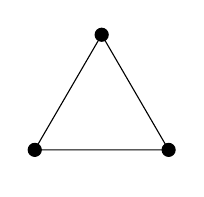
\begin{tikzpicture}[%
x={(1.7cm,0cm)},
y={(0cm,1.7cm)},
]

\coordinate (A) at (0,0); 
\coordinate (B) at (1,0) ;
\coordinate (C) at (0.5,0.86); 

%Ecken
\node[circle,scale=0.5,fill=black,draw=black](Ap) at (0,0){};
\node[circle,scale=0.5,fill=black,draw=black](Bp) at (1,0){};
\node[circle,scale=0.5,fill=black,draw=black](Cp) at (0.5,0.86){};

%Kanten
\draw[] (A)
-- (B)  node[midway, below]{}
-- (C)      node[midway, right]{}
-- (A)  node[midway, left]{};

\end{tikzpicture}
\subcaption{}
\end{minipage}
\hfill
 \begin{minipage}[t]{.2\textwidth}
   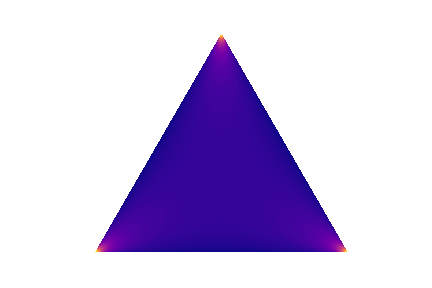
\includegraphics[width=\textwidth]{plots/notebooks/gs1.png}
\subcaption{}
\end{minipage}
\hfill
 \begin{minipage}[t]{.2\textwidth}
   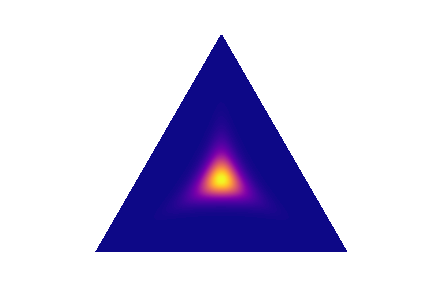
\includegraphics[width=\textwidth]{plots/notebooks/gs5.png}
\subcaption{}
\end{minipage}
\hfill
 \begin{minipage}[t]{.2\textwidth}
   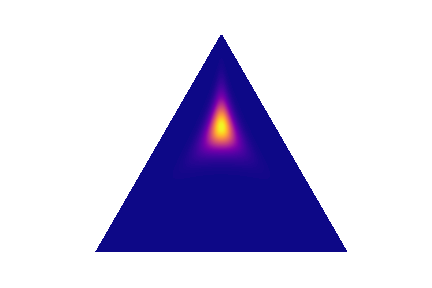
\includegraphics[width=\textwidth]{plots/notebooks/gs5_shift.png}
\subcaption{}
\end{minipage}

\caption{Пример распределения Gumbel-Softmax при различных значениях параметров: а)~$\lamT\to0$, б)~$\lamT=1, \s=[1,1,1]$, в)~$\lamT=5, \s=[1,1,1]$, г)~$\lamT=5, \mathbf{s}=[10,0.1,0.1].$}
\label{fig:gs}

\end{figure}


Заметим, что предлагаемое априорное распределение неоднозначно: одно и то же распределение  можно получить с различными значениями гиперпарамета $\mathbf{A}^{j,k}_l$ и структурного параметра $\gamma^{j,k}_l$. В качестве регуляризатора для матрицы $(\mathbf{A}^{j,k}_l)^{-1}$ предлагается использовать обратное гамма-распределение:
\[
    (\A^{j,k}_l)^{-1} \sim \text{inv-gamma}(\lambda_1,\lambda_2),
\]
где $\lambda_1,\lambda_2 \in \lam$ --- метапараметры оптимизации. 
Использование обратного гамма-распределения в качестве распределения гиперпараметров можно найти в~\cite{bishop,mackay}. В данной работе обратное распределение выступает как регуляризатор гиперпараметров.
Варьируя метапарамы $\lambda_1,\lambda_2$ получается  более сильная или более слабая регуляризация~\cite{rvm}. Пример распределений $\text{inv-gamma}(\lambda_1,\lambda_2)$ для разных значений метапараметров $\lambda_1,\lambda_2$ изображен на Рис.~\ref{fig:inv-gamma}. Оптимизации без регуляризации соответствует случай предельного распределения $\lim_{\lambda_1,\lambda_2\to 0}\text{inv-gamma}(\lambda_1, \lambda_2)$.

\begin{figure}
\centering
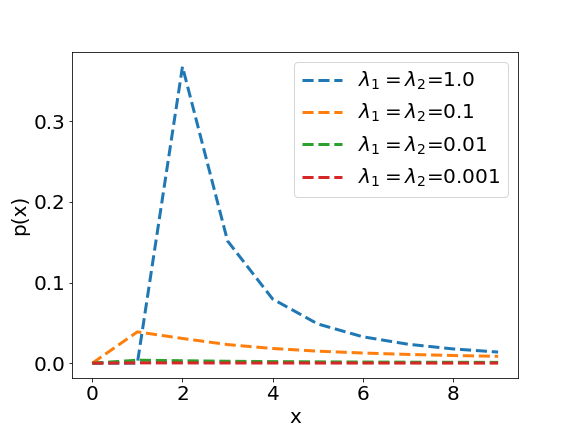
\includegraphics[width=0.6\textwidth]{plots/notebooks/invgamma.png}
\caption{Графики обратных гамма распределений для различных значений метапараметров.}
\label{fig:inv-gamma}
\end{figure}


Таким образом, предлагаемая вероятностная модель содержит следующие компоненты:
\begin{enumerate}
\item Параметры $\w$ модели, распределенные нормально.
\item Структура модели $\G$, содержащая все структурные параметры $\{\g^{j,k}, (j,k) \in E\}$ распределены по распределению Gumbel-Softmax.
\item Гиперпараметры: $\h = [\text{diag}(\A), \s]$, где $\A$ --- конкатенация матриц $\A^{j,k}, (j,k) \in E,$ $\s$ --- конкатенация параметров Gumbel-Softmax распределений $\s^{j,k}, (j,k) \in E$, где $E$ --- множество ребер, соответствующих графу рассматриваемого параметрического семейства.
\item Метапараметры: $\lam = [\lambda_1, \lambda_2, \lamT].$ Эти параметры не подлежат оптимизации и задаются экспертно. 
\end{enumerate}

График вероятностной модели в формате плоских нотаций представлен на Рис.~\ref{fig:plate_prob}.
\begin{figure}
\centering
   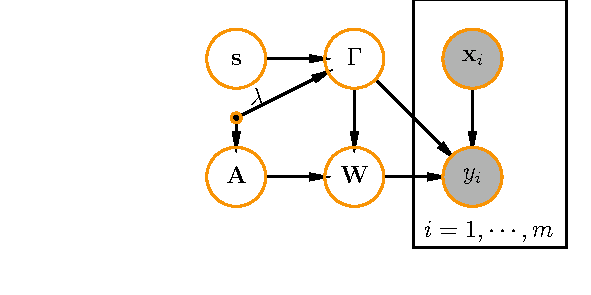
\includegraphics[width=0.5\textwidth]{plots/notebooks/simple_plate.pdf}
\caption{График предлагаемой вероятностной модели в формате плоских нотаций. Переменные обозначены белыми и серыми кругами, константы обозначены обведенными черными кругами. Наблюдаемые переменные обозначены серыми кругами.}
\label{fig:plate_prob}
\end{figure}

\section{Вариационная оценка для обоснованности вероятностной модели}
В качестве критерия выбора структуры модели предлагается использовать апостериорную вероятность гиперпараметров:
\begin{equation}
\label{eq:optimal_hyper}
    \posth \propto \EV \priorh \to \max_{\h \in \Hb},
\end{equation}
где структура модели и параметры модели выбираются на основе полученных значений гиперпараметров:
\[
    \G^* = \argmax_{\G \in \Gb} p(\G|\y, \X, \h^*, \lam ),
\]
\[
    \w^* = \argmax_{\w \in \Wb} p(\w|\y, \X, \G^*, \g^*),
\]
где $\h^*$ --- решение задачи оптимизации~\eqref{eq:optimal_hyper}.

Для вычисления обоснованности $$\EV = \iint_{\G, \w}\LL \priorw \priorG d\G d\w$$ из~\eqref{eq:optimal_hyper} предлагается использовать вариационную оценку обоснованности.

\begin{theorem}
Пусть $\q = \qw \qG$ --- вариационное распределение c параметрами $\teta= [\tetaw, \tetaG ]$, аппроксимирующее апостериорное распределение структуры и параметров:
\[
    \q \approx \post,
\]
\[
    \qw  \approx \postw,
\]
\[
    \qG \approx \qG.
\]

Тогда справедлива следующая оценка:
\begin{equation}
\label{eq:full_elbo}
\log \EV \geq
\end{equation}
\[
 \E_{\G \sim \qG} \E_{\w \sim \qw} \log \LL - \KL{\qG}{\priorG} - 
\]
\[
 - \KL{\qw}{\priorw},
\]
где $\KL{\qw}{\priorw}$ вычисляется по формуле условной дивергенции~\cite{TODO}:
\[
\KL{\qw}{\priorw} = \E_{\G \sim \qG} \E_{\w \sim \qw} \log \left(\frac{\qw)}{\priorw}\right).
\]
\end{theorem}

\begin{proof}
Рассмотрим обоснованность:
\[
\log \EV  =  \log \iint_{\G,\w} \LL \priorw \priorG d\G d\w  =
\]
\[
   = \log\iint_{\G,\w} \LL \priorw \frac{\q}{\q}d\G d\w =
\]
\[
  =  \log \E_{\q} \frac{\EV}{\q}.
\]
Используя неравенство Йенсена получим 
\[
 \log \E_{\q} \frac{\EV}{\q} \geq
\]
\[
 \geq  \E_{\q} \log \LL - \KL{\q}{\prior}.
\]
Декомпозируем распределение $q$ по свойству условной дивергенции:
\[
\KL{\q}{\prior} = 
\]
\begin{equation}
\label{eq:kl_full}
= \KL{\qG}{\priorG} + \E_{\G \sim \qG} \E_{\w \sim \qw} \log \left(\frac{\qw)}{\priorw}\right).    
\end{equation}
\end{proof}
В качестве вариационного распределения $\qw$ предлагается использовать нормальное распределение, не зависящее от структуры модели $\G$:
\[
    \qw  \sim \mathcal{N}(\boldsymbol{\mu}_q, \A_q), 
\]
где $\A_q$ --- диагональная матрица с диагональю $\boldsymbol{\alpha}_q$.

В качестве вариационного распределения $\qG$ предлагается использовать произведение распределений Gumbel-Softmax. Конкатенацию параметров концентрации распределений обозначим $\s_q$. Его температуру, общую для всех структурных параметров $\g \in \G$, обозначим $\theta_\text{temp}$.
Вариационными параметрами распределения $\q$ являются параметры распределений $\qw, \qG$:
\[\teta =[\boldsymbol{\mu}_q, \boldsymbol{\alpha}_q,\s_q, \theta_\text{temp}]. 
\]
График вероятностной вариационной модели в формате плоских нотаций представлен на Рис.~\ref{fig:plate_qprob}.
\begin{figure}
\centering
   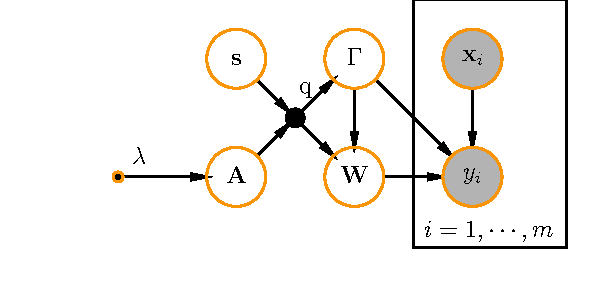
\includegraphics[width=0.5\textwidth]{plots/notebooks/plate.pdf}
\caption{График предлагаемой вероятностной вариационной модели в формате плоских нотаций. Переменные обозначены белыми и серыми кругами, константы обозначены обведенными черными кругами. Вариационное распределение обозначено черным кругом. Наблюдаемые переменные обозначены серыми кругами.}
\label{fig:plate_qprob}
\end{figure}

Для анализа сложности полученной модели введем понятие \textit{параметрической сложности}. 
\begin{defin} 
Параметрической сложностью  $C_p(\teta|\Uh, \lam)$ модели с вариационными параметрами $\teta$ на компакте $\Uh \subset \Hb$ назовем минимальную дивергенцию между вариационным и априорным распределением:
\[
C_p(\teta|\Uh, \lam) = \min_{\h \in \Uh} \KL{\q}{\prior}.
\]
\end{defin}
Параметрическая сложность модели соответствует минимальной по $\h \in \Uh$ ожидаемой длине описания параметров модели при условии заданного параметрического априорного распределения~\cite{hinton_mdl}.

Одним из критериев удаления неинформативных параметров в вероятностных моделях является отношение вариационной плотности параметров в моде распределения к вариационной плотности параметра в нуле~\cite{nips}:
\[\frac{\qw[w=\mu_q]}{\qw[w=0]}= \text{exp}\left(-\frac{2\alpha_q^2}{\mu_q^2}\right),
\]
где $\qw[w] \sim \mathcal{N}(\mu_q, \alpha_q).$

Обобщим понятие относительной вариационной плотности на случай произвольных непрерывных распределений.
\begin{defin}
Относительной вариационной   плотностью параметра $w \in \w$  при условии структуры $\G$ и гиперпараметров $\h$ назовем отношение вариационной плотности в моде вариационного распределения параметра к вариационной плотности в моде априорного распределению параметра:
\[
\rho(w|\G,\tetaw, \h,\Lamb)=\frac{\qw[\text{mode}\qw]}{\qw[\text{mode}~\priorw]}.
\]
Относительной вариационной плотностью вектора параметров $\mathbf{w}$ назовем следующее выражение:
\[
    \boldsymbol{\rho}(\w|\G, \tetaw, \h,\lam) = \prod_{w \in \w}\rho(w|\G,\tetaw,\h,\lam).
\]

\end{defin}

Сформулируем и докажеми теорему о связи относительной плотности и параметрической сложности модели:

\begin{theorem}
Пусть
\begin{enumerate}
\item заданы компактные множества $\Uh \subset \Hb, \Utetaw \subset \Tetawb, \UtetaG \subset \TetaGb$;


\item Мода априорного распределения $\prior$ не зависит от гиперпараметров $\h$  на $\Uh$ и структуры $\G$ на $\UtetaG$:
\[
\text{mode}~\priorw[][\G_1][\h_1]=\text{mode}~\priorw[][\G_1][\h_2]=\mathbf{M}~\forall~\h_1,\h_2 \in \Uh, \G_1,\G_2 \in \UG;
\]

\item вариационное распределение $\qw$ и априорное распределение $\priorw$  являются абсолютно непрерывными и унимодальными на  $U_\mathbf{h}, U_{\boldsymbol{\theta}}$;

\item вариационное распределение $\qw$ является липшецевым по $\w$;

\item значение $\qw[\mathbf{M}]$ не равно нулю при $\teta \in \Uteta$;

\item Решение задачи вида 
\begin{equation}
\label{eq:dkl_solve}
\h^{*} = \argmin_{\h \in \Uh} \KL{\q}{\prior}
\end{equation} единственно для любого $\teta \in \Uteta$.
\item Параметры модели $\w$ имеют конечные вторые моменты по распределениям:
\[
   \int_{\G}\qG\qw d\G, \quad \int_{\G}\qG\priorw d\G;
\]

\item мода и матожидание вариационного распределения $\qw$ и априорного распределения $\priorw$  совпадают:
\[
    \text{mode}~\priorw= \E_{\priorw} \w;
\]
\[
  \text{mode}~\qw = \E_{\qw} \w;
\]

\item задана  бесконечная последовательность векторов вариационных параметров $\teta_1,\teta_2,\dots,\teta_i \in \Uteta$, такая что $\lim_{i \to \infty}C_p(\teta_i|\Uh,\lam) = 0.$

\end{enumerate}
Тогда следующее выражение стремится к единице:
\[
   \E_{\qG} \boldsymbol{\rho}(\w|\G, \tetaw, \h, \lam) \to 1.
\]


\end{theorem}

\begin{proof}
Обозначим за $\h_i$ --- решение задачи~\eqref{eq:dkl_solve} для вектора вариационных параметров $\teta_i$.
Воспользуемся неравенством Пинскера:
\[
    ||F_q(\teta_i)-F_p(\h_i)||_\text{TV},\leq\sqrt{2\KL{\q[\teta_i]}{\prior[][][\h_i]}},
\]
где $||\cdot||_\text{TV}$ --- расстояние по вариации, $F_q, F_p$ --- функции распределения   $\q[\teta_i],\prior[][][\h_i].$
Т.к. дивергенция~\eqref{eq:kl_full} состоит из двух неотрицательных величин, то обе они стремятся к нулю.
Рассмотрим вторую величину:
%\E_{\G \sim \qG} \E_{\w \sim \qw} \log \left(\frac{\qw)}{\priorw}\right)
\[
  0 =   \lim_{i \to \infty} \E_{\G \sim \qG} \E_{\w \sim \qw} \log \left(\frac{\qw)}{\priorw}\right) = 
\]
\[
 \lim_{i \to \infty} |\int_{\G} \int_{\w} \log \left(\frac{\qw)}{\priorw}\qG\qw d\w d\w\right) | \geq   \lim_{i \to \infty} \geq 
\]
\[
 \lim_{i \to \infty} \geq \int_{\G} ||F_q(\teta_i)-F_p(\h_i)||_\text{TV}\qG d\G.  
\]
Отсюда $ \lim_{i \to \infty} ||F_q(\teta)-F_p(\h)||_\text{TV} = 0.$
По теореме Шеффе данное выражение можно переписать как:
\[
    \lim_{i \to \infty}   \frac{1}{2}\iint_{\w,\G} |\priorw - \qw| \qG d\G d\w = 0.
\]

Для произвольного $\teta$ рассмотрим выражение:
\[
   \left|\int_{\G} \frac{\qw[\text{mode}\qw]}{\qw[\text{mode}\priorw]} -  \frac{\qw[\E_{\qw} \w]}{[\qw[\mathbf{M}]} \qG d\G \right| =
\]
\[  \left|\int_{\G} \frac{\qw[\E_{\qw}\w]}{\qw[\mathbf{M}]} -  \frac{\qw[\E_{\qw} \w]}{[\qw[\mathbf{M}]}\qG d\G\right| \leq 
\]
\[
\int_{\G} \left|\frac{\qw[\E_{\qw} \w)]}{{\qw[\mathbf{M}]}} -   \frac{\qw[\E_{\qw} \w]}{[\qw[\mathbf{M}]}\qG d\G\right| \leq
\]
\[
\frac{C_l}{\min_{\tetaw \in \Uteta} \qw[\mathbf{M}]}\int_{\G}  |\E_{\qw}\w - \E_{\priorw}\w|\qG d\G  \leq
\]
\[
    \leq \frac{C_l}{\min_{\tetaw \in \Uteta} \qw[\mathbf{M}]} \iint_{\G,\w} |\w| |\qw - \priorw|\qG d\w d\G,
\]
где $C_l$ --- максимальная константа Липшица для $\qw$ на $\Uteta$. 
%https://math.stackexchange.com/questions/112786/convergence-in-law-and-uniformly-integrability
Определим случайную величину $\boldsymbol{\nu}(t), t \geq 0$ следующим образом:
\[
    \boldsymbol{\nu}(t) = \boldsymbol{\max}(-t \cdot \mathbf{1}, \boldsymbol{\min}(t \cdot \mathbf{1}, \w)).
\]
Данная величина совпадает с $\w$ при $|\w| < t$ и принимает значение $t$ или $-t$ при $|\w| \geq t$,
Тогда для любого $t>0$ справедливо:
\[
    \iint_{\G,\w} |\w| |\qw - \priorw|\qG d\w d\G \leq
\]
\[ 
\leq  \iint_{\G,\w} |\w -\boldsymbol{\nu}(t)| |\qw - \priorw|\qG d\w d\G   +
\]
\[
 +    \iint_{\G,\w} |\boldsymbol{\nu}(t)||\priorw-\qw|d\w \leq
\]
\begin{equation}
\label{eq:tmp}
    \leq    \iint_{\G,\w} |\w -\boldsymbol{\nu}(t)|\priorw -\qw| d\w d\G   +
\end{equation}
\[ +      \iint_{\G,\w} |\boldsymbol{\nu}(t)| |\qw - \priorw|\qG d\w d\G.
\]

ассмотрим первое слагаемое суммы~\eqref{eq:tmp}. Т.к. вторые моменты $\E_{\qG}\E_{\qw} \w^2, \E_{\qG}{\priorw} \w^2$ конечны, то случайная величина $\w$ равномерно интегрируема как при маргинальном распределении $\int_{\G}\qG\qw d\G$, так и при маргинальном распределении $\int_{\G}\qG\priorw d\G$.
По определению равномерной интегрируемости для $\w$ для любого числа $\varepsilon$ существует число $t_0$, такое что для любого $t \geq t_0$ справедливо выражение:
\[
    \E|\w - \boldsymbol{\nu}(t)| d\w d\G \leq \varepsilon.
\]
где матожидание берется по  распределениям $\int_{\G}\qG\qw d\G$,$\int_{\G}\qG\priorw d\G$. Тогда
\[
   \iint_{\G,\w} |\w -\boldsymbol{\nu}(t)|\priorw  - \qw| d\w d\G   \leq  
\]
\[
  \iint_{\G,\w} |\w -\boldsymbol{\nu}(t)|\priorw  +   \iint_{\G,\w} |\w -\boldsymbol{\nu}(t)|\qw d\G d\w
\]
для любого $t$. Устремляя $t$ к бесконечности, получим $$\lim_{i \to \infty}     \iint_{\G,\w} |\w -\boldsymbol{\nu}(t)|\priorw  - \qw| d\w d\G = 0.$$

Рассмотрим второе слагаемое. 
Т.к. $|\boldsymbol{\nu}(t)|$ --- ограничена, то 
\[
      \iint_{\G,\w} |\boldsymbol{\nu}(t)| |\qw - \priorw|\qG d\w d\G   \leq
\]
\[
\leq t  \iint_{\G,\w} |\qw - \priorw|\qG d\w d\G.
\]
Данное выражение стремится к нулю при $i \to \infty$.

Таким образом выражение $\left|\int_{\G} \frac{\qw[\text{mode}\qw]}{\qw[\text{mode}\priorw]}\qG d\G \right|$ стремится к единице, что и требовалось доказать.
\end{proof}

Теорема утверждает, что при устремлении параметрической сложности модели к нулю, все параметры модели подлежат удалению в среднем по всем возможным значениям  структуры $\G$ модели. Заметим, что теорема применима для случая, когда последовательность вариационных распределений $q$ не имеет предела. Так, в случае, если структура $\G$ определена однозначно, последовательность $\teta_i$ может являться последовательностью нормальных распределений, чье матожидание стремится к нулю:
\[
    \teta_i \sim \mathcal{N}((\boldsymbol{\mu}_q)_i, (\A^{-1}_q)_i), (\boldsymbol{\mu}_q)_i \to \mathbf{0}.
\]
Априорным распределением $\prior = \priorw$ при этом может являться семейство нормальных распределений с нулевым средним:
\[
    \priorw = \mathcal{N}(\mathbf{0}, \A^{-1}).
\]
При этом сама последовательность распределений $\teta_i$ не обязана иметь предел.

\section{Обобщающая задача}
В данном разделе проводится анализ основных критериев выбора моделей, а также предлагается их обобщение на случай моделей, испольюзующих вариационное распределение $\q$ для аппроксимации неизвестного апостериорного распределения параметров $\prior$.

Рассмотрим основные статистические критерии выбора вероятностных моделей. 
\begin{enumerate}
\item Критерий максимального правдоподобия:
\[\log \LL \to \max_{\w \in \Uw, \G \in \UG}.\]
Для использования данного критерия в качестве задачи выбора модели предлагается следующее обобщение:
\begin{equation}
\label{eq:optim_ml}
    \Loss =  \E_{\q} \log~\LL.
\end{equation}
Данное обобщение~\eqref{eq:optim_ml} эквивалентно  критерию правдоподобия при выборе в качестве $\q$ эмпирического распределения парамтетров и структуры.
Метод не предполагает оптимизации гиперпараметров $\h$. Для формального соответствия данной задачи задаче выбора модели~\eqref{TOD}, т.е. двухуровневой задачи оптимизации, положим $\Loss=\Val:$
\[
    \Loss =  \E_{\q}\log \LL \to \max_{\teta},
\]
\[
    \Val =  \E_{\q}\log \LL \to \max_{\h},
\]



\item Метод максимальной апостериорной вероятности. 
\[\log \LL \prior \to \max_{\w  \in \Uw, \G \in \UG}.\]
Аналогично предыдущему методу сформулируем вариационное обобщение данной задачи:
\begin{equation}
\label{eq:optim_map}
\Loss = \Val = \E_{\q} \bigl( \log\LL + \log\prior \bigr).
\end{equation}
Т.к. в рамках данной задачи~\eqref{eq:optim_map} не предполагается оптимизации гиперпараметров $\h$, положим параметры распределения $\prior$ фиксированными:
\[
   \lam = [\lambda_1, \lambda_2, \lamT, \s, \text{diag}(\A)].
\]

\item Перебор структуры:
\begin{equation}
\label{eq:optim_struct}
    \Loss = \Val = \E_{\q} \log \LL [\qG = p']
\end{equation}
где $p'$ --- некоторое распределение на структуре $\G$, выступающее в качестве метапараметра.




\item Критерий Акаике:
\[
   \text{AIC} =  \log \LL |\Wb|.
\]
Т.к. все рассматриваемые модели принадлежат одному параметрическому семейству моделей $\F$, то количество параметров у всех рассматриваемых моделей  совпадает. Тогда критерий Акаике совпадает с критерием максимального правдоподобия. Для использования критерия Акаике для сравнения моделей, принадлежащих одному параметрическому семейству~$\F$ предлагается следующая переформулировка:
\begin{equation}
\label{eq:optim_aic}
    \Loss = \Val = \log \LL - |\{w: \KL{\teta}{\h}<\lambda_\text{prune}\}|,
\end{equation}
где 
\begin{equation}\label{eq:aic_compl}\h=\argmin_{\h' \in \Uh} \KL{\q}{\prior},\end{equation} $\lambda_{\text{prune}}$ --- метапараметр алгоритма, $\Uh  \subset \Hb$ --- область определения задачи по гиперпараметрам. Предложенное обобщение~\eqref{eq:optim_aic} применимо только в случае, если выражение~\eqref{eq:aic_compl} определено однозначно, т.е. существует единственный вектор гиперпараметров на $\Uh,$ доставляющий минимум дивергенции $\KL{\q,\prior}.$

\item Информационный критерий Шварца:
\[
    \text{BIC} = \log \LL -0.5\log(m)|\Wb|.
\]
Переформулируем данный критерий аналогично критерию AIC:
\begin{equation}
\label{eq:optim_bic}
    \Loss = \Val = BIC_{\lambda} = \log \LL - \log m |\{w: \KL{\q}{\h}<\lambda_{\text{prune}}\}|,
\end{equation}
метапараметр $\lambda_{\text{prune}}$ определен аналогично~\eqref{eq:aic_compl}.

\item Метод вариационной оценки обоснованности:
\begin{equation}
\label{eq:optim_elbo_method}   
    \Loss = \E_{\q} \log \LL - \KL{\q,\prior} + \priorh \to \max_{\teta},
\end{equation}
\[
     \Loss = \E_{\q} \log \LL - \KL{\q,\prior} + \priorh \to \max_{\h},
\]
В рамках данной задачи функции $\Loss$ и $\Val$ совпадают, все гиперпараметры $\h$ подлежат оптимизации.

\item Валидация на отложенной выборке:
\begin{equation}
\label{eq:optim_hold_out}
    \Loss = \E_{\q} \log \LL + \prior \to \teta,
\end{equation}
\[
    \Val = \E_{\q} \log \LL \to \max_{h},
\]
где $(\X_\text{train}, \y_\text{train}), (\X_\text{test}, \y_\text{test})$ --- разбиение выборки на обучающую и контрольную подвыборку.
В рамках данной задачи, все гиперпараметры $\h$ подлежат оптимизации.

\end{enumerate}

Каждый из рассмотренных критерии удовлетворяет хотя бы одному из перечисленных свойств:
\begin{enumerate}[label={\arabic*)}]
\item модель, оптимизируемая согласно критерию, доставляет максимум правдоподобия выборки;
\item модель, оптимизируемая согласно критерию, доставляет максимум оценки обоснованности;
\item для моделей, доставляющих сопоставимые значения правдоподобия выборки, выбирается модель с меньшим количеством информативных параметров.
\item критерий позволяет производить перебор структур для отбора наилучших модели.
\end{enumerate}

Формализуем рассмотренные критерии. Оптимизационную задачу, которая удовлетворяет всем перечисленным свойствам при некоторых значинях метапараметров, будет называть \textit{обобщающей}.

\begin{defin}
Двухуровневую задачу оптимизации будем называть \textit{обобщающей} на компакте $U = \Uteta \times \Uh \times \Uh \times \Ulam \subset \Tetab \times \Hb \times \Lamb$, если она удовлетворяет следующим критериям.
\begin{enumerate}
\item Область определения каждого параметра $w \in \w$, гиперпараметра $h \in \h$ и метапараметра $\lambda \in \lam$ не  является пустым множеством и не является точкой.
\item Для каждого значения гиперпараметров $\h$ оптимальное решение нижней~\eqref{TODO} задачи оптимизации 
\[
\teta^{*}(\h) = \argmax_{\teta \in \Tetab} \Loss
\]
определено однозначно при любых значениях метапараметров $\lam \in \Ulam$.

\item Критерий максимизации правдоподобия выборки: существует $\lam \in \Ulam$ и  $$K_1>0, \quad K_1 < \max_{\h_1,\h_2 \in \Uh} \Val[\h_1][][][\teta^{*}(\h_1)] - \Val[\h_2][][][\teta^{*}(\h_2)],$$ такие что для любых векторов гиперпараметров, удовлетворяющих неравенству $$\h_1, \h_2 \in \Uh, \Val[\h_1][][][\teta^{*}(\h_1)] - \Val[\h_2][][][\teta^{*}(\h_2)] > K_1,$$ выполняется неравенство $$\E_{\q[\teta^{*}(\h_1)]}\LL > \E_{\q[\teta^{*}(\h_2)]}\LL$$.

\item Критерий минимизации параметрической сложности:  существует  $\lam \in \Ulam$ и $$K_2>0, \quad K_2 < \max_{\h_1, \h_2 \in \Uh} \Val[\h_1][][][\teta^{*}(\h_1)] - \Val[\h_2][][][\teta^{*}(\h_2)],$$ такие что для любых векторов гиперпараметров $\h_1,\h_2 \in \Uh$, удовлетворяющих неравенству $$\Val[\h_1][][][\teta^{*}(\h_1)] - \Val[\h_2][][][\teta^{*}(\h_2)]>K_2,$$ параметрическая сложность первой модели меньше, чем второй: $$C_p(\teta^{*}(\h_1)|\Uh,\lam)<C_p(\teta^{*}(h_2)|\Uh,\lam).$$

\item Критерий приближения оценки обоснованности: существует значение гиперпараметров $\lam$, такое что значение функций потерь $\Loss$ и валидации $\Val$ пропорционален вариационной оценки обоснованности модели: $$\Loss \propto  \Val \propto $$
$$\propto
\E_{\q}\LL - \KL{\q}{\prior} + \log\priorh$$ для всех $\teta \in \Uteta, \h \in \Uh.$ 

\item Критерий перебора оптимальных структур: существует набор метапараметров $\lam$ и константа $$K_3>0, \quad K_3 < \max_{\mathbf{h}_1, \mathbf{h}_2} \KL{\priorG[][\h_1]}{\priorG[][\h_2]},\KL{\priorG[][\h_2]}{\priorG[][\h_1]},$$ такие что для локальных оптимумов задачи оптимизации $\h_1,\h_2$, полученных при метапараметрах $\lam$ и удовлетворяющих неравенствам $$\KL{\priorG[][\h_1]}{\priorG[][\h_2]} > K_3, \KL{\priorG[][\h_2]}{\priorG[][\h_1]}>K_3,$$  существует значение метапараметров $\lam'$, такие что
\begin{enumerate}
\item Соответствие между вариационными параметрами $\teta^{*}(\h_1),\teta^{*}(\h_2)$ сохраняется при  $\lam'$.
\item  $\Val[\h_1] < \Val[\h_2]$ при $\lam'$.
\end{enumerate}


\item Критерий нерперывности: функции $\Loss$ и $\Val$ непрерывны по метапараметрам $\lam \in \Ulam$.
\end{enumerate}
\end{defin}
Первый критерий является техническим и используется для исключения из рассмотрения вырожденных задач оптимизации.  
Второй критерий говорит о том, что решение первого и второго уровня должны быть согласованы и определены однозначно.
Критерии 3-5 определяют возможные критерии оптимизации, которые должны приближаться обобщающей задачей.
Критерий 6 говорит о возможности перехода между различными структурами модели. Данный критерий говорит о том, что мы можем перейти от одного набора гиперпараметров $\h_1$ к другим $\h_2$, если они соответствуют локальным оптимумам задачи оптимизации, и дивергенция соответствующих априорных  распределений на структурах $\priorG$ значимо высока. При этом соответствующие вариационные распределения $\qG$ могут оказаться достаточно близки. Возможным дополнением этого критерия был бы критерий, позволяющий переходить от структуры к структуре, если соответствующие распределения $\qG$ различаются значимо.
Последний критерий говорит о том, что обобщающая задача должна позволять производить переход между различными методами выбора  параметров и структуры модели непрерывно.

\begin{theorem}Рассмотренные задачи~\eqref{eq:optim_ml},\eqref{eq:optim_map},\eqref{eq:optim_struct},\eqref{eq:optim_aic},\eqref{eq:optim_bic},\eqref{eq:optim_hold_out} не являются обобщающими.
\end{theorem}
\begin{proof}
Задачи~\eqref{eq:optim_ml},\eqref{eq:optim_map},\eqref{eq:optim_struct},\eqref{eq:optim_aic},\eqref{eq:optim_bic} не имеют гиперпараметров $\mathbf{h}$, подлежащих оптимизации, поэтому не могут оптимизировать вариационную оценку.

При  использовании валидации на отложенной выборки~\eqref{eq:optim_hold_out} в функцию валидации $\Val$ не входит ни один метапараметр, поэтому критерий перебора структур 6 для нее также не выполняется. 

\end{proof}

\begin{theorem}
Пусть $q_{\boldsymbol{\Gamma}}$ --- абсолютно непрерывное распределение с дифференцируемой плотностью, такой что:
\begin{enumerate}
\item градиент плотности $\nabla_{\boldsymbol{\theta}_{\boldsymbol{\Gamma}}} q(\boldsymbol{\Gamma}|\boldsymbol{\theta}_{\boldsymbol{\Gamma}})$ является нулевым не более чем счетное количество раз. 
\item выражение $\nabla_{\boldsymbol{\theta}_{\boldsymbol{\Gamma}}} q(\boldsymbol{\Gamma}|\boldsymbol{\theta}_{\boldsymbol{\Gamma}}) \text{log}p(\boldsymbol{\Gamma}|\mathbf{h}, \boldsymbol{\lambda})$ ограничено на $U_{\boldsymbol{\theta}}$ некоторой случайной величиной с конечным первым моментом.
\end{enumerate}
Тогда задача~\eqref{eq:optim_elbo_method} не является обобщающей.
\end{theorem}
\begin{proof}
Пусть выполнены условия критерия 6 о переборе структур, и $\mathbf{h}_1, \mathbf{h}_2$ --- локальные оптимумы функции $\Val$ при метапараметрах $\boldsymbol{\lambda}$.
По условию критерия соответствтие $\boldsymbol{\theta}^{*}(\mathbf{h}_1)$ и $\boldsymbol{\theta}^{*}(\mathbf{h}_2)$ должны сохраняться, т.е. для некоторого $\boldsymbol{\lambda}'$ решение  нижней задачи оптимизации $\boldsymbol{\theta}^{*}(\mathbf{h}_1)$ должно совпадать с решением $\boldsymbol{\theta}^{*}(\mathbf{h}_1)$ при метапараметрах $\boldsymbol{\lambda}$. Тогда
\[
    \nabla_{\boldsymbol{\theta}} \mathsf{E}_{q(\mathbf{w}, \boldsymbol{\Gamma}|\boldsymbol{\theta}_1)} \text{log}~p(\mathbf{y}|\mathbf{X}, \mathbf{w}, \boldsymbol{\Gamma}) -\nabla_{\boldsymbol{\theta}}  \text{D}_{\text{KL}}(q(\mathbf{w}, \boldsymbol{\Gamma}|\boldsymbol{\theta}_1) | p(\mathbf{w}, \boldsymbol{\Gamma}|\mathbf{h}_1, \boldsymbol{\lambda})) = 
\]
\[
= \nabla_{\boldsymbol{\theta}} \mathsf{E}_{q(\mathbf{w}, \boldsymbol{\Gamma}|\boldsymbol{\theta}_1)} \text{log}~p(\mathbf{y}|\mathbf{X}, \mathbf{w}, \boldsymbol{\Gamma}) - \nabla_{\boldsymbol{\theta}}  \text{D}_{\text{KL}}(q(\mathbf{w}, \boldsymbol{\Gamma}|\boldsymbol{\theta}_1) | p(\mathbf{w}, \boldsymbol{\Gamma}|\mathbf{h}_1, \boldsymbol{\lambda}')).
\]
Сокращая равные слагаемые в равенстве получим:
\[
\nabla_{\boldsymbol{\theta}}  \text{D}_{\text{KL}}(q(\boldsymbol{\Gamma}|\boldsymbol{\theta}_1) | p(\boldsymbol{\Gamma}| \boldsymbol{\lambda})) = \nabla_{\boldsymbol{\theta}} \text{D}_{\text{KL}}(q(\boldsymbol{\Gamma}|\boldsymbol{\theta}_1) | p(\boldsymbol{\Gamma}| \boldsymbol{\lambda}')),
\] 
Из второго условия теоремы следует, что по теореме Лебега о мажорируемой сходимости осуществим переход дифференцирования под знак интеграла:
\[
\int_{\boldsymbol{\Gamma} \in \amsmathbb{\Gamma}} \nabla_{\boldsymbol{\theta}_\Gamma} q(\boldsymbol{\Gamma}|\boldsymbol{\theta}_2) (\text{log}~p(\boldsymbol{\Gamma}| \boldsymbol{\lambda}) - \text{log}~p(\boldsymbol{\Gamma}| \boldsymbol{\lambda}')) d\boldsymbol{\Gamma} = 0.
\]
Т.к. выражение $ \nabla_{\boldsymbol{\theta}_\Gamma} q(\boldsymbol{\Gamma}|\boldsymbol{\theta}_2)$ принимает нулевое значение в счетном количестве точек, то выражение $\text{log}~p(\boldsymbol{\Gamma}| \boldsymbol{\lambda}) - \text{log}~p(\boldsymbol{\Gamma}| \boldsymbol{\lambda}')$ равно нулю почти всюду, что означает что метапараметр температуры $\lambda_\text{temp}$  равен при разных значениях метапараметров:
\[
\lambda_\text{temp} = \lambda_\text{temp}',\quad \lambda_\text{temp} \in \boldsymbol{\lambda}, \lambda_\text{temp}' \in \boldsymbol{\lambda}'.
\]
Таким образом, метапараметры $\boldsymbol{\lambda},\boldsymbol{\lambda}'$ отличаются лишь на метапараметры  $\lambda_1, \lambda_2$ регуляризации ковариационной матрицы~$\mathbf{A}^{-1}$. 
Возьмем в качестве векторов гиперпараметров $\mathbf{h}_1,\mathbf{h}_2$ гиперпараметры, отличающиеся только параметрами распределения структуры:
\[
    \mathbf{h}_1 = [\mathbf{s}_1, \text{diag}(\mathbf{A}_1)], \mathbf{h}_2 = [\mathbf{s}_2, \text{diag}(\mathbf{A}_2)],\quad \mathbf{s}_1 \neq \mathbf{s}_2, \mathbf{A}_1 = \mathbf{A}_2.
\]
Метапараметры $\lambda_1, \lambda_2$ не влияют на значение функции $\Val$ при гиперпараметрах, отличающихся только параметрами распределения структуры, поэтому значение функции $Q$ для них будет неизменно при любых значениях $\lambda_1, \lambda_2$. Приходим к противоречию: значение $\Val$ не меняется при изменении метапараметров $\boldsymbol{\lambda}$.

\end{proof}
\iffalse
В качестве обобщающей задачи оптимизации предлагается оптимизационную задачу следующего вида:
\begin{equation}
\label{eq:qopt}
\mathbf{h}^{*} = \argmax_{\mathbf{h}} Q = 
\end{equation}
\[
= {\lambda_\text{likelihood}^\text{Q}\mathsf{E}_{{q}^{*}} \text{log}~{p(\mathbf{y} | \mathbf{X}, \mathbf{w},\boldsymbol{\Gamma}, \mathbf{h}, \lambda_\text{temp}, \mathbf{f})}}
 -\]
\vspace{-0.3cm}
\[- {\lambda^\text{prior}_\text{Q}\text{D}_{KL}\bigl( q^{*}(\mathbf{w}, \boldsymbol{\Gamma}) || p(\mathbf{w}, \boldsymbol{\Gamma} |\mathbf{h}, \lambda_{\text{temp}},\mathbf{f}) \bigr)}  -\]
\vspace{-0.3cm}
\[
-{\sum_{p' \in \mathbf{P}, \lambda \in \boldsymbol{\lambda}^\text{struct}_\text{Q}} \lambda\text{D}_{KL}(\boldsymbol{\Gamma} | p')+\text{log}p(\mathbf{h}|\mathbf{f})}, 
\]
\begin{equation}
\tag{$L^{*}$}
{q}^{*} = \argmax_{q} L = 
{\mathsf{E}_q \text{log}~{p(\mathbf{y} | \mathbf{X}, \mathbf{w}, \boldsymbol{\Gamma}, \mathbf{h}, \lambda_{\text{temp}}, \mathbf{f})}}
\end{equation}
\vspace{-0.3cm}
\[- {\lambda^\text{prior}_\text{L}\text{D}_{KL}\bigl( q^{*}(\mathbf{w}, \boldsymbol{\Gamma}) || p(\mathbf{w}, \boldsymbol{\Gamma} |\mathbf{h}, \lambda_{\text{temp}},\mathbf{f}) \bigr)},
\]
где $\mathbf{P}$ --- непустое множество распределений на структуре $\boldsymbol{\Gamma}$, $\lambda^\text{prior}_\text{Q}, \lambda_\text{likelihood}^\text{Q}, \boldsymbol{\lambda}^\text{struct}_\text{Q}$ --- некоторые числа. Множество распределений $\mathbf{P}$ отвечает за перебор структур $\boldsymbol{\Gamma}$ в процессе оптимизации модели. Подробное объяснение данного множества дано ниже. 


\begin{theorem}
Пусть:
\begin{enumerate}[label={\arabic*)}] 
\item задано непустое множество непрерывных по параметрам распределений на структуре $\mathbf{P}$, где хотя бы одно распределение принадлежит Gumbel-Softmax-распределению.

\item вариационное распределение $q = q_{\boldsymbol{\Gamma}}(\boldsymbol{\Gamma}|\boldsymbol{\theta}_{\boldsymbol{\Gamma}}) q_{\mathbf{w}}(\mathbf{w}| \boldsymbol{\Gamma},\boldsymbol{\theta}_{\boldsymbol{\Gamma}})$ является  абсолютно непрерывным, плотность которого непрерывна по метапараметрам $\boldsymbol{\lambda}$;

\item задан компакт  $U = U_{\boldsymbol{\theta}} \times U_{\mathbf{h}} \times U_{\boldsymbol{\lambda}} \subset \amsmathbb{\Theta} \times \mathbb{H} \times \amsmathbb{\Lambda}$, где параметры распределений $\mathbf{P} \in \amsmathbb{\Lambda}$, область $U_{\boldsymbol{\theta}}$ декомпозируется на две области $U_{\boldsymbol{\theta}} = U_{\boldsymbol{\theta}_{\mathbf{w}}} \times U_{\boldsymbol{\theta}_{\boldsymbol{\Gamma}}}$;

\item область определения каждого параметра $w \in \mathbf{w}$, гиперпараметра $h \in \mathbf{h}$ и метапараметра $\lambda \in \boldsymbol{\lambda}$ не является является пустым и не является точкой;

\item для каждого значения гиперпараметров $\mathbf{h}$ оптимальное решение нижней задачи оптимизации $\boldsymbol{\theta}^{*}$ определено однозначно при любых значениях метапараметров $\boldsymbol{\lambda} \in U_{\lambda}$;

\item область значений метапараметров $\lambda_\text{likelihood}^\text{Q}, \lambda^\text{prior}_\text{Q}, \boldsymbol{\lambda}^\text{struct}_\text{Q}, \lambda^\text{prior}_\text{L}$ включает отрезок от нуля до единицы;

\item существует значение метапараметров $\lambda_1, \lambda_2, \lambda_\text{likelihood}^\text{Q}$, такое что
\[
\max_{\mathbf{h}} \text{log} p (\mathbf{h}|\boldsymbol{\lambda})-\min_{\mathbf{h}} \text{log}~p(\mathbf{h}|\boldsymbol{\lambda}) < \max_{\mathbf{h}} Q(\mathbf{h}) -  \min_{\mathbf{h}} Q(\mathbf{h}).
\] 
при $\boldsymbol{\lambda}^\text{struct}_Q = \mathbf{0}, \lambda^\text{prior}_Q = 0$.

\item существует значение метапараметров $ \lambda^\text{prior}_\text{Q}, \lambda_1, \lambda_2, \lambda_\text{temp}$, такое что 
\[
    \max_{\mathbf{h}} \text{log}~p (\mathbf{h}|\boldsymbol{\lambda}) - \min_{\mathbf{h}} \text{log}~p (\mathbf{h}|\boldsymbol{\lambda})  + \max_{\mathbf{h}} \min_{\boldsymbol{\theta}} D_\text{KL}(q(\mathbf{w}, \boldsymbol{\Gamma}|\boldsymbol{\theta})|p(\mathbf{w}, \boldsymbol{\Gamma}|\mathbf{h}, \boldsymbol{\lambda})) -
\]
\[ \min_{\mathbf{h}, \boldsymbol{\theta}} D_\text{KL}(q(\mathbf{w}, \boldsymbol{\Gamma}|\boldsymbol{\theta})|p(\mathbf{w}, \boldsymbol{\Gamma}|\mathbf{h}, \boldsymbol{\lambda})) + \max_{\boldsymbol{\theta}}\frac{1}{\lambda^\text{prior}_\text{L}}\mathsf{E}_q(\mathbf{w}, \boldsymbol{\Gamma}|\boldsymbol{\theta}) \text{log} p(\mathbf{y}|\mathbf{X}, \mathbf{w})  - 
\]
\[
 - \min_{\boldsymbol{\theta}}\frac{1}{\lambda^\text{prior}_\text{L}}\mathsf{E}_q(\mathbf{w}, \boldsymbol{\Gamma}|\boldsymbol{\theta}) \text{log} p(\mathbf{y}|\mathbf{X}, \mathbf{w}) < \max_{\boldsymbol{\theta}, \mathbf{h}} D_{\text{KL}} - \min_{\boldsymbol{\theta}, \mathbf{h}} D_{\text{KL}}.
\]

\item существуют значения метапараметров $\lambda^\text{prior}_\text{Q},\lambda^\text{likelihood}_\text{Q}, \lambda_1, \lambda_2, \lambda_\text{temp},$ такие что 
\[
\max_{\mathbf{h}} D_{\text{KL}} - \min_{\mathbf{h}} D_{\text{KL}} < \frac{\max_{\mathbf{h}} Q - \min_{\mathbf{h}} Q }{\max_{\lambda_\text{struct}}} 
\]
при $\boldsymbol{\lambda}^\text{struct}_\text{Q} = 0.$

\end{enumerate}
Тогда задача~\eqref{eq:qopt} является обобщающей на $U$.
\end{theorem}
\begin{proof}
Для доказательста теоремы требуется доказать критерии 1-7 из определения обобщающей задачи.
Выполнение критериев 1 и 2 следует из условий задачи.

Докажем критерий 3. 
Пусть $\lambda^{\text{prior}}_\text{Q} = 0, \boldsymbol{\lambda}^\text{struct}_\text{Q} = \mathbf{0}$. 
Пусть $\lambda_1, \lambda_2, \lambda_\text{likelihood}^\text{Q}$ удовлетворяют седьмому условияю теоремы.
Возьмем в качестве $K_1$ следующее выражение:
\[
    K_1= \max_{\mathbf{h}} \text{log} p (\mathbf{h}|\boldsymbol{\lambda})-\min_{\mathbf{h}} \text{log}~p(\mathbf{h}|\boldsymbol{\lambda}).
\]
Пусть $\mathbf{h}_1, \mathbf{h}_2 \in U_\mathbf{h}, Q(\mathbf{h}_1)-Q(\mathbf{h}_2)>K_1$.
Тогда 
\[
Q(\mathbf{h}_1)-Q(\mathbf{h}_2) = \lambda^\text{likelihood}_\text{Q} \mathsf{E}_{q(\mathbf{w}, \boldsymbol{\Gamma}|\boldsymbol{\theta}_1)} \text{log}~p(\mathbf{y}|\mathbf{X}, \mathbf{w}, \boldsymbol{\Gamma})-\]
\[
-\lambda^\text{likelihood}_\text{Q}  \mathsf{E}_{q(\mathbf{w}, \boldsymbol{\Gamma}|\boldsymbol{\theta}_2)} \text{log}~p(\mathbf{y}|\mathbf{X}, \mathbf{w}, \boldsymbol{\Gamma})
+\text{log}~p(\mathbf{h}_2|\boldsymbol{\lambda})-\text{log}~p(\mathbf{h}_1|\boldsymbol{\lambda})>K_1.
\]
Отсюда следует  выполнение критерия 3:
\[
\lambda^\text{likelihood}_\text{Q} \mathsf{E}_{q(\mathbf{w}, \boldsymbol{\Gamma}|\boldsymbol{\theta}_1)} \text{log}~p(\mathbf{y}|\mathbf{X}, \mathbf{w}, \boldsymbol{\Gamma}) - \lambda^\text{likelihood}_\text{Q} \mathsf{E}_{q(\mathbf{w}, \boldsymbol{\Gamma}|\boldsymbol{\theta}_2)} \text{log}~p(\mathbf{y}|\mathbf{X}, \mathbf{w}, \boldsymbol{\Gamma}) > 0.
\]

Докажем критерий 4. 
Пусть $\boldsymbol{\lambda}$ удовлетворяют восьмому условию и $\lambda^{\text{likelihood}}_\text{Q} = 0, \boldsymbol{\lambda}^\text{struct}_\text{Q} = \mathbf{0}$.
Пусть 
\[
K_2 =  \max_{\mathbf{h}} \text{log}~p (\mathbf{h}|\boldsymbol{\lambda}) - \min_{\mathbf{h}} \text{log}~p (\mathbf{h}|\boldsymbol{\lambda})  + \max_{\mathbf{h}} \min_{\boldsymbol{\theta}} D_\text{KL}(q(\mathbf{w}, \boldsymbol{\Gamma}|\boldsymbol{\theta})|p(\mathbf{w}, \boldsymbol{\Gamma}|\mathbf{h}, \boldsymbol{\lambda})) -
\]
\[ \min_{\mathbf{h}, \boldsymbol{\theta}} D_\text{KL}(q(\mathbf{w}, \boldsymbol{\Gamma}|\boldsymbol{\theta})|p(\mathbf{w}, \boldsymbol{\Gamma}|\mathbf{h}, \boldsymbol{\lambda})) + \max_{\boldsymbol{\theta}}\frac{1}{\lambda^\text{prior}_\text{L}}\mathsf{E}_q(\mathbf{w}, \boldsymbol{\Gamma}|\boldsymbol{\theta}) \text{log} p(\mathbf{y}|\mathbf{X}, \mathbf{w})  - 
\]
\[
 - \min_{\boldsymbol{\theta}}\frac{1}{\lambda^\text{prior}_\text{L}}\mathsf{E}_q(\mathbf{w}, \boldsymbol{\Gamma}|\boldsymbol{\theta}) \text{log} p(\mathbf{y}|\mathbf{X}, \mathbf{w}).
\]
Пусть $\mathbf{h}_1, \mathbf{h}_2 \in U_\mathbf{h}, Q(\mathbf{h}_1)-Q(\mathbf{h}_2)>K_1$.
Рассмотрим разность параметрических сложностей двух векторов:
\[
C_p(\boldsymbol{\theta}_2)-C_p(\boldsymbol{\theta}_1) = \min_{\mathbf{h}} D_\text{KL}(q(\mathbf{w}, \boldsymbol{\Gamma}|\boldsymbol{\theta}_2)|p(\mathbf{w}, \boldsymbol{\Gamma}|\mathbf{h}, \boldsymbol{\lambda})) - 
\]
\[
-\min_{\mathbf{h}} D_\text{KL}(q(\mathbf{w}, \boldsymbol{\Gamma}|\boldsymbol{\theta}_1)|p(\mathbf{w}, \boldsymbol{\Gamma}|\mathbf{h}, \boldsymbol{\lambda})) \geq
\]
% добавляем D_kl вместо D_KL^*
\[
\geq
\min_{\mathbf{h}} D_\text{KL}(q(\mathbf{w}, \boldsymbol{\Gamma}|\boldsymbol{\theta}_2)|p(\mathbf{w}, \boldsymbol{\Gamma}|\mathbf{h}, \boldsymbol{\lambda}))- D_\text{KL}(q(\mathbf{w}, \boldsymbol{\Gamma}|\boldsymbol{\theta}_1)|p(\mathbf{w}, \boldsymbol{\Gamma}|\mathbf{h}_1, \boldsymbol{\lambda})) +
\]
\[
+D_\text{KL}(q(\mathbf{w}, \boldsymbol{\Gamma}|\boldsymbol{\theta}_2)|p(\mathbf{w}, \boldsymbol{\Gamma}|\mathbf{h}_2, \boldsymbol{\lambda})) - D_\text{KL}(q(\mathbf{w}, \boldsymbol{\Gamma}|\boldsymbol{\theta}_2)|p(\mathbf{w}, \boldsymbol{\Gamma}|\mathbf{h}_2, \boldsymbol{\lambda})) =
\]
% Доводим до Q
\[
= Q(\mathbf{h}_1)-Q(\mathbf{h}_2)-\text{log}~p (\mathbf{h}_1|\boldsymbol{\lambda})+\text{log}~p (\mathbf{h}_2|\boldsymbol{\lambda})+
\]
\[+\min_{\mathbf{h}} D_\text{KL}(q(\mathbf{w}, \boldsymbol{\Gamma}|\boldsymbol{\theta}_2)|p(\mathbf{w}, \boldsymbol{\Gamma}|\mathbf{h}, \boldsymbol{\lambda})) -  D_\text{KL}(q(\mathbf{w}, \boldsymbol{\Gamma}|\boldsymbol{\theta}_1)|p(\mathbf{w}, \boldsymbol{\Gamma}|\mathbf{h}_1, \boldsymbol{\lambda})) >
\]
% Доводим до K_2
\[
>K_2 -\text{log}~p (\mathbf{h}_1|\boldsymbol{\lambda})+\text{log}~p (\mathbf{h}_2|\boldsymbol{\lambda}) + \min_{\boldsymbol{\theta}, \mathbf{h}} D_\text{KL}(q(\mathbf{w}, \boldsymbol{\Gamma}|\boldsymbol{\theta})|p(\mathbf{w}, \boldsymbol{\Gamma}|\mathbf{h}, \boldsymbol{\lambda})) 
\]
\[
-  D_\text{KL}(q(\mathbf{w}, \boldsymbol{\Gamma}|\boldsymbol{\theta}_1)|p(\mathbf{w}, \boldsymbol{\Gamma}|\mathbf{h}_1, \boldsymbol{\lambda})).
\]
Рассмотрим разность:
\[\min_{\boldsymbol{\theta}, \mathbf{h}} D_\text{KL}(q(\mathbf{w}, \boldsymbol{\Gamma}|\boldsymbol{\theta})|p(\mathbf{w}, \boldsymbol{\Gamma}|\mathbf{h}, \boldsymbol{\lambda}))  - D_\text{KL}(q(\mathbf{w}, \boldsymbol{\Gamma}|\boldsymbol{\theta}_1)|p(\mathbf{w}, \boldsymbol{\Gamma}|\mathbf{h}_1, \boldsymbol{\lambda})) =
\]
\[
= \min_{\boldsymbol{\theta}, \mathbf{h}} D_\text{KL}(q(\mathbf{w}, \boldsymbol{\Gamma}|\boldsymbol{\theta})|p(\mathbf{w}, \boldsymbol{\Gamma}|\mathbf{h}, \boldsymbol{\lambda}))  - \frac{1}{\lambda^\text{prior}_\text{L}}\mathsf{E}_q(\mathbf{w}, \boldsymbol{\Gamma}|\boldsymbol{\theta}_1) \text{log} p(\mathbf{y}|\mathbf{X}, \mathbf{w}) +
\]
\[
+ \max_{\boldsymbol{\theta}}  (\frac{1}{\lambda^\text{prior}_\text{L}}\mathsf{E}_{q(\mathbf{w}, \boldsymbol{\Gamma}|\boldsymbol{\theta})} \text{log} p(\mathbf{y}|\mathbf{X}, \mathbf{w}) - D_\text{KL}(q(\mathbf{w}, \boldsymbol{\Gamma}|\boldsymbol{\theta})|p(\mathbf{w}, \boldsymbol{\Gamma}|\mathbf{h}_1, \boldsymbol{\lambda}))) \geq
\]
% взяли максимум от правдоподобия
\[
    \geq \min_{\boldsymbol{\theta}, \mathbf{h}} D_\text{KL}(q(\mathbf{w}, \boldsymbol{\Gamma}|\boldsymbol{\theta})|p(\mathbf{w}, \boldsymbol{\Gamma}|\mathbf{h}, \boldsymbol{\lambda})) - \max_{\boldsymbol{\theta}}\frac{1}{\lambda^\text{prior}_\text{L}}\mathsf{E}_q(\mathbf{w}, \boldsymbol{\Gamma}|\boldsymbol{\theta}) \text{log} p(\mathbf{y}|\mathbf{X}, \mathbf{w}) +
\]
\[ + \max_{\boldsymbol{\theta}}  (\min_{\boldsymbol{\theta}'} \frac{1}{\lambda^\text{prior}_\text{L}}\mathsf{E}_{q(\mathbf{w}, \boldsymbol{\Gamma}|\boldsymbol{\theta'})} \text{log} p(\mathbf{y}|\mathbf{X}, \mathbf{w}) - D_\text{KL}(q(\mathbf{w}, \boldsymbol{\Gamma}|\boldsymbol{\theta})|p(\mathbf{w}, \boldsymbol{\Gamma}|\mathbf{h}_1, \boldsymbol{\lambda})))  \geq
\]
% добавили минимум под максимум
\[
 \geq
\min_{\boldsymbol{\theta}, \mathbf{h}} D_\text{KL}(q(\mathbf{w}, \boldsymbol{\Gamma}|\boldsymbol{\theta})|p(\mathbf{w}, \boldsymbol{\Gamma}|\mathbf{h}, \boldsymbol{\lambda})) - \max_{\boldsymbol{\theta}}\frac{1}{\lambda^\text{prior}_\text{L}}\mathsf{E}_q(\mathbf{w}, \boldsymbol{\Gamma}|\boldsymbol{\theta}) \text{log} p(\mathbf{y}|\mathbf{X}, \mathbf{w}) +
\]
\[
+ \min_{\boldsymbol{\theta}} \frac{1}{\lambda^\text{prior}_\text{L}}\mathsf{E}_{q(\mathbf{w}, \boldsymbol{\Gamma}|\boldsymbol{\theta})} \text{log} p(\mathbf{y}|\mathbf{X}, \mathbf{w}) 
- \min_{\boldsymbol{\theta}} D_\text{KL}(q(\mathbf{w}, \boldsymbol{\Gamma}|\boldsymbol{\theta})|p(\mathbf{w}, \boldsymbol{\Gamma}|\mathbf{h}_1, \boldsymbol{\lambda}))) 
 \geq
\]
% Взяли оценку от всех выражений
\[
 \geq
\min_{\boldsymbol{\theta}, \mathbf{h}} D_\text{KL}(q(\mathbf{w}, \boldsymbol{\Gamma}|\boldsymbol{\theta})|p(\mathbf{w}, \boldsymbol{\Gamma}|\mathbf{h}, \boldsymbol{\lambda})) - \max_{\boldsymbol{\theta}}\frac{1}{\lambda^\text{prior}_\text{L}}\mathsf{E}_q(\mathbf{w}, \boldsymbol{\Gamma}|\boldsymbol{\theta}) \text{log} p(\mathbf{y}|\mathbf{X}, \mathbf{w}) +
\]
\[ + \min_{\boldsymbol{\theta}} \frac{1}{\lambda^\text{prior}_\text{L}}\mathsf{E}_{q(\mathbf{w}, \boldsymbol{\Gamma}|\boldsymbol{\theta})} \text{log} p(\mathbf{y}|\mathbf{X}, \mathbf{w}) 
- \max_{\mathbf{h}}\min_{\boldsymbol{\theta}} D_\text{KL}(q(\mathbf{w}, \boldsymbol{\Gamma}|\boldsymbol{\theta})|p(\mathbf{w}, \boldsymbol{\Gamma}|\mathbf{h}, \boldsymbol{\lambda}))). 
\]
Складывая полученную оценку с $K_2 -\text{log}~p (\mathbf{h}_2|\boldsymbol{\lambda})+\text{log}~p (\mathbf{h}_1|\boldsymbol{\lambda})$ получаем разность параметрических сложностей больше нуля.

Докажем критерий 5. Пусть $\lambda^\text{likelihood}_\text{Q} = \lambda^\text{prior}_\text{L} = \lambda^\text{prior}_\text{Q} > 0$, $\boldsymbol{\lambda}^\text{struct}_\text{Q} = \mathbf{0}$. Тогда функции $L$ и $Q$  можно записать как: $$L = Q \propto \left(\mathsf{E}_q p(\mathbf{y}|\mathbf{w}, \mathbf{X})-{D}_{KL}(q(\mathbf{w}, \boldsymbol{\Gamma}|\boldsymbol{\theta})|p(\mathbf{w}, \boldsymbol{\Gamma}|\mathbf{h}, \boldsymbol{\lambda}))\right),$$ что и требовалось доказать.

Докажем критерий 6. 
Пусть задан вектор метапараметров~$\boldsymbol{\lambda}$, удовлетворяющий девятому условию теоремы и $\boldsymbol{\lambda} = \mathbf{0}$. 
Возьмем в качестве $K_4$ следующее выражение:
\[
K_4 = \frac{\max_{\mathbf{h}} Q - \min_{\mathbf{h}} Q }{\max_{\lambda_\text{struct}}}.
\]



Пусть вектор метапараметров $\boldsymbol{\lambda}'$ отличается от $\boldsymbol{\lambda}$ лишь метапараметром $\boldsymbol{\lambda}_\text{struct}$. Для  обоих векторов метапараметров нижняя задача  оптимизации $L$ совпадает, поэтому выполняется первое условие критерия.

Без ограничения общности предположим, что $Q(\mathbf{h}_1)-Q(\mathbf{h}_2) > 0$ при $\boldsymbol{\lambda}.$ Также без ограничения общности будем полгаать, что множестве $\mathbf{P}$ состоит только из одного распределения на структуре $\boldsymbol{\Gamma}$, равного распределению на структуре $p(\boldsymbol{\Gamma}|\mathbf{h}_1, \boldsymbol{\lambda}).$
%Положим распределение из $\mathbf{P}$ имеющим то же распределение, что и априорное $\mathbf{P} = \{p'(\boldsymbol{\Gamma})\}, p(\boldsymbol{\Gamma}) \sim \text{GS}(\mathbf{s}', \lambda_\text{temp}')\}$. 

Положим для $\boldsymbol{\lambda}'$ параметр $\lambda_\text{struct}$ равным максимальному значению: $\lambda_\text{struct} = \max \lambda_\text{struct}'$.
Тогда при $\boldsymbol{\lambda}'$ неравенство 
\[\
Q(\mathbf{h}_1|\boldsymbol{\lambda}')-Q(\mathbf{h}_2|\boldsymbol{\lambda}')  = Q(\mathbf{h}_1|\boldsymbol{\lambda})-Q(\mathbf{h}_2|\boldsymbol{\lambda})  + \lambda'_\text{struct} D_\text{KL}(p(\boldsymbol{\Gamma}|\mathbf{h}_2,\boldsymbol{\lambda}')|p(\boldsymbol{\Gamma}|\mathbf{h}_1,\boldsymbol{\lambda}')) >
\]
\[
  > Q(\mathbf{h}_1|\boldsymbol{\lambda})-Q(\mathbf{h}_2|\boldsymbol{\lambda})  +  \lambda'_\text{struct}K_4   = Q(\mathbf{h}_1|\boldsymbol{\lambda})-Q(\mathbf{h}_2 + |\boldsymbol{\lambda})  + \max_{\mathbf{h}} Q - \min_{\mathbf{h}} Q   =0,
\]
что и требовалось доказать.

Докажем критерий 7. Достаточным условием непрерывности функций $L$, $Q$ является непрерывность входящих в нее слагаемых. 
Т.к. априорные распределения задаются нерперывными функциями плотности $p(\mathbf{w}|\boldsymbol{\Gamma},\mathbf{h}), p(\boldsymbol{\Gamma}|\mathbf{h},\boldsymbol{\lambda})$, и функция плотности $p(\boldsymbol{\Gamma}|\mathbf{h},\boldsymbol{\lambda})$ распределения структуры $\boldsymbol{\Gamma}$ ограничена на компакте, то дивергенция $D_\text{KL}(q(\mathbf{w}, \boldsymbol{\Gamma}|\boldsymbol{\theta})|p(\mathbf{w}, \boldsymbol{\Gamma}|\mathbf{h},\boldsymbol{\lambda})$ непрерывна по метапараметрам.
Т.к. остальные слагаемые функций оптимизаций $L,Q$ также непрерывны по метапараметрам, то непрерывна и сами функции оптимизации.
\end{proof}

Метапараметрами данной задачи~\eqref{eq:qopt} являются коэффициенты $\lambda^\text{prior}_\text{Q}, \lambda^\text{prior}_\text{L}$, отвечающие за регуляризацию верхней и нижней задачи оптимизации, коэффициент $\lambda_\text{likelihood}^\text{Q}$ отвечает за максимизацию правдоподобия, а также параметры распрделений $\mathbf{P}$ и вектор коэффициентов перед ними $\boldsymbol{\lambda}^\text{struct}_\text{Q}$. 

В предельном случае, когда температура $\lambda_\text{temp}$ близка к нулю, а множество $\mathbf{P}$ состоит из распределений, близких к дискретным,а соответствующим всем возможным структурам, калибровка $\boldsymbol{\lambda}^\text{struct}_\text{Q}$ порождает последовательность задач оптимизаций, схожую с перебором структур. Рассмотрим следующий пример. 

\begin{example} 
Рассмотрим вырожденный случай поведения функции $Q$, когда $\lambda_\text{likelihood}^\text{Q} = \lambda^\text{prior}_\text{Q} = 0$. Пусть модель использует один структурный параметр, в качестве априорного распределения на структуре задано распределение Gumbel-Softmax с $\lambda_\text{temp}=1.0$. Пусть в качестве множества распределений $\mathbf{P}$ используется два распределения Gumbel-Softmax, сконцентрированных близко к вершинам симплекса:
\[
    \mathbf{P} = [\mathcal{GS}([0.95, 0.05, 0.05]^\text{T}, 1.0) ,\mathcal{GS}([0.95, 0.05, 0.05]^{\text{T}}, 1.0)].
\]
Из определения распределения Gumbel-Softmax следует, что достаточно рассмотреть только значения параметра $\mathbf{s}$ ,находящиеся внутри симплекса.
На рис.~\ref{fig:gs_comb} изображены значения функции Q в зависимости от метапараметров $\boldsymbol{\lambda}^\text{struct}_\text{Q}$ и значений гиперпараметра $\mathbf{s}$ распределения на структуре. Видно, что варьируя  коэффициенты метапараметров получается последовательность оптимизаций, схожая с полным перебором структуры.
\end{example}


\begin{figure}
 \begin{minipage}[t]{.32\textwidth}
   \includegraphics[width=\textwidth]{plots/notebooks/struct_reg_1.png}
\subcaption{}
\end{minipage}
\hfill
 \begin{minipage}[t]{.32\textwidth}
   \includegraphics[width=\textwidth]{plots/notebooks/struct_reg_2.png}
\subcaption{}
\end{minipage}
\hfill
 \begin{minipage}[t]{.32\textwidth}
   \includegraphics[width=\textwidth]{plots/notebooks/struct_reg_3.png}
\subcaption{}
\end{minipage}

\caption{Пример зависимости функции $Q$ от гиперпараметра $\mathbf{s}$ при различных значениях метапараметров $\boldsymbol{\lambda}^\text{struct}_Q$. Темные точки на графике соответсвуют наименее предпочтительным значениям гиперпараметра. а)~$\boldsymbol{\lambda}^\text{struct}_Q = [0,0],$ б)~$~\boldsymbol{\lambda}^\text{struct}_Q = [1,0],$ в)~$~\boldsymbol{\lambda}^\text{struct}_Q = [1,1].$}
\label{fig:gs_comb}

\end{figure}

\section{Анализ обобщающей задачи}
В данном разделе рассматриваются свойства предложенной задачи при различных значениях метапараметров, а также характер ассимптотического поведения задач.


\begin{theorem}
Пусть $m \gg 0$, ${\lambda_\text{prior}^L} > 0, \frac{m}{\lambda_\text{prior}^L}   \in \mathbb{N}, \frac{m}{\lambda_\text{prior}^L}  \gg 0.$ Тогда оптимизация функции
\[
L = 
{\mathsf{E}_q \text{log}~{p(\mathbf{y} | \mathbf{X}, \mathbf{w}, \boldsymbol{\Gamma})}}-{\lambda_\text{prior}^L \text{D}_{KL}(q(\mathbf{w}, \boldsymbol{\Gamma}|\boldsymbol{\theta})||p(\mathbf{w}, \boldsymbol{\Gamma} |\mathbf{h}, \lambda_{\text{temp}})}
\] эквивалентна оптимизации вариационной оценки обоснованности  $\mathsf{E}_q \text{log}~{p(\hat{\mathbf{y}} | \hat{\mathbf{X}}, \mathbf{w}, \boldsymbol{\Gamma}, \mathbf{h}, \lambda_{\text{temp}},\mathbf{f})} - \text{D}_{KL}(q(\mathbf{w}, \boldsymbol{\Gamma}|\boldsymbol{\theta})||p(\mathbf{w}, \boldsymbol{\Gamma} |\mathbf{h}, \lambda_{\text{temp}})$
для произвольной случайной подвыборки $\hat{\mathbf{y}}, \hat{\mathbf{X}}$ мощности $\frac{m}{{\lambda_\text{prior}^L}}$ из генеральной совопкупности.
\end{theorem}
\begin{proof}
Рассмотрим величину  $\frac{1}{m}L$: \\
\begin{equation}
\label{eq:l_m}
    \frac{1}{m}L = \frac{1}{m}\mathsf{E}_q \text{log}p(\mathbf{y}|\mathbf{X},  \mathbf{w}, \boldsymbol{\Gamma}, \mathbf{h}, \boldsymbol{\lambda})-\frac{\lambda_\text{prior}^L}{m}D_\text{KL}(q(\mathbf{w}, \boldsymbol{\Gamma}|\boldsymbol{\theta})|p(\mathbf{w},\boldsymbol{\Gamma}|\mathbf{h}, \boldsymbol{\lambda})).
\end{equation}

При $m \gg 0$ по усиленному закону больших чисел данная функция эквивалентна:
\[
    \frac{1}{m}L \approx  \mathsf{E}_{y, \mathbf{x}} \mathsf{E}_{q} \text{log}p(y|\mathbf{x}, \mathbf{w}, \boldsymbol{\Gamma}, \mathbf{h}, \boldsymbol{\lambda}) -\frac{\lambda_\text{prior}^L}{m}D_\text{KL}(q(\mathbf{w}, \boldsymbol{\Gamma}|\boldsymbol{\theta})|p(\mathbf{w},\boldsymbol{\Gamma}|\mathbf{h}, \boldsymbol{\lambda})).
\]

Аналогично рассмотрим вариационную оценку обоснованности для произвольной выборки мощностью $m_0 = \frac{m}{\lambda_\text{prior}^L}$, усредненную на мощность выборки:
\begin{equation}
\label{eq:l_m0}
    \frac{1}{m_0}\mathsf{E}_q \text{log}p(\mathbf{y}|\mathbf{X},  \mathbf{w}, \boldsymbol{\Gamma}, \mathbf{h}, \boldsymbol{\lambda})-\frac{1}{m_0}D_\text{KL}(q(\mathbf{w}, \boldsymbol{\Gamma}|\boldsymbol{\theta})|p(\mathbf{w},\boldsymbol{\Gamma}|\mathbf{h}, \boldsymbol{\lambda})) \approx
\end{equation}
\[
\approx  \mathsf{E}_{y, \mathbf{x}} \mathsf{E}_{q} \text{log}p(y|\mathbf{x}, \mathbf{w}, \boldsymbol{\Gamma}, \mathbf{h}, \boldsymbol{\lambda}) -\frac{1}{m_0}D_\text{KL}(q(\mathbf{w}, \boldsymbol{\Gamma}|\boldsymbol{\theta})|p(\mathbf{w},\boldsymbol{\Gamma}|\mathbf{h}, \boldsymbol{\lambda})) = 
\]
\[
= \mathsf{E}_{y, \mathbf{x}} \mathsf{E}_{q} \text{log}p(y|\mathbf{x}, \mathbf{w}, \boldsymbol{\Gamma}, \mathbf{h}, \boldsymbol{\lambda}) -\frac{\lambda_\text{prior}^L}{m}D_\text{KL}(q(\mathbf{w}, \boldsymbol{\Gamma}|\boldsymbol{\theta})|p(\mathbf{w},\boldsymbol{\Gamma}|\mathbf{h}, \boldsymbol{\lambda})).
\]
Таким образом, задачи оптимизации функций~\eqref{eq:l_m},\eqref{eq:l_m0} совпадают, что и требовалось доказать.
\end{proof}
Таким образом, для достаточно большого $m$ и $\lambda^{\text{prior}}_L>0, \lambda^{\text{prior}}_L \neq 1$ оптимизация параметров и гиперпараметров эквивалентна нахождению оценки обоснованности для выборки другой мощности: чем выше значение $ \lambda^{\text{prior}}_L$, тем выше мощность выборки, для которой проводится оптимизация.


Следующие теоремы говорят о соответствии предлагаемой обобщающей задачи вероятностной модели. В частности, задача оптимизации параметров и гиперпараметров соответствует двухуровневому байесовскому выводу.
\begin{theorem}
Пусть ${\lambda^Q_\text{likelihood}} = {\lambda^L_\text{prior}=\lambda^Q_\text{prior}}=1, {\boldsymbol{\lambda}^Q_{\text{struct}}}=\mathbf{0}$. Тогда:
\begin{enumerate}
\item Задача оптимизации~\eqref{eq:qopt} доставляет максимум апостериорной вероятности гиперпараметров с использованием вариационной оценки обоснованности:
\vspace{-0.3cm}
\[
    \text{log}\hat{p}(\mathbf{y}|\mathbf{X}, \mathbf{h}, \lambda_\text{temp}, \mathbf{f})+{\text{log}p(\mathbf{h}|\mathbf{f})} \to \max_{\mathbf{h}}.
\]
\item Вариационное распределение $q$ приближает апостериорное распределение $p(\mathbf{w}, \boldsymbol{\Gamma}|\mathbf{y}, \mathbf{X}, \mathbf{h}, \boldsymbol{\lambda}, \mathbf{f})$ наилучшим образом:
\vspace{-0.3cm}
\[
    {D}_\text{KL}(q(\mathbf{w}, \boldsymbol{\Gamma}|\boldsymbol{\theta})|p(\mathbf{w}, \boldsymbol{\Gamma}|\mathbf{y}, \mathbf{X}, \mathbf{h}, \boldsymbol{\lambda})) \to \min_{\boldsymbol{\theta}}.
\]


\item Если существуют такие значения параметров $\boldsymbol{\theta}_\mathbf{w}, \boldsymbol{\theta}_{\boldsymbol{\Gamma}},$ что $p(\boldsymbol{\Gamma}|\mathbf{y}, \mathbf{X}, \mathbf{h}, \boldsymbol{\lambda}) = q(\boldsymbol{\Gamma}|\boldsymbol{\theta}_{\boldsymbol{\Gamma}})$, $p(\mathbf{w}| \mathbf{y}, \mathbf{X}, \boldsymbol{\Gamma}, \mathbf{h}, \boldsymbol{\lambda}) = q(\mathbf{w}|\boldsymbol{\Gamma}, \boldsymbol{\theta}_{\mathbf{w}})$,
то решение задачи оптимизации $L$ доставляет эти значения вариационных параметров.  
\end{enumerate}
\end{theorem}
\begin{proof}
При $\lambda^Q_\text{likelihood} = \lambda^L_\text{prior} = 1$ как верхняя, так и нижняя задачи оптимизации~\eqref{eq:qopt} эквивалентны оптимизации вариационной оценки обоснованности, поэтому первое утверждение выполняется.

Докажем второе утвреждение. Рассмотрим логарифм обоснованности модели: 
\[
\text{log} p(\mathbf{y}|\mathbf{X}, \mathbf{h}, \boldsymbol{\lambda}) = \mathsf{E}_q \text{log}\frac{p(\mathbf{y}|\mathbf{x}, \mathbf{w}, \boldsymbol{\Gamma})p(\mathbf{w}, \boldsymbol{\Gamma}|\mathbf{h}, \boldsymbol{\lambda})}{q(\mathbf{w}, \boldsymbol{\Gamma}| \boldsymbol{\theta})} +
\]
\[
+ {D}_\text{KL}(q(\mathbf{w}, \boldsymbol{\Gamma}|\boldsymbol{\theta})|p(\mathbf{w}, \boldsymbol{\Gamma}|\mathbf{y}, \mathbf{X}, \mathbf{h}, \boldsymbol{\lambda})) = 
\]
\[
 \mathsf{E}_q \text{log} p(\mathbf{y}|\mathbf{x}, \mathbf{w}, \boldsymbol{\Gamma}) -{D}_\text{KL}(q(\mathbf{w}, \boldsymbol{\Gamma}|\boldsymbol{\theta})|p(\mathbf{w}, \boldsymbol{\Gamma}|\mathbf{h}, \boldsymbol{\lambda})) + {D}_\text{KL}(q(\mathbf{w}, \boldsymbol{\Gamma}|\boldsymbol{\theta})|p(\mathbf{w}, \boldsymbol{\Gamma}|\mathbf{y}, \mathbf{X}, \mathbf{h}, \boldsymbol{\lambda})).
\]
Из данного равенства следует:
\[
\text{log} p(\mathbf{y}|\mathbf{X}, \mathbf{h}, \boldsymbol{\lambda}) - {D}_\text{KL}(q(\mathbf{w}, \boldsymbol{\Gamma}|\boldsymbol{\theta})|p(\mathbf{w}, \boldsymbol{\Gamma}|\mathbf{y}, \mathbf{X}, \mathbf{h}, \boldsymbol{\lambda})) =
\]
\[
    \mathsf{E}_q \text{log} p(\mathbf{y}|\mathbf{x}, \mathbf{w}, \boldsymbol{\Gamma}) -{D}_\text{KL}(q(\mathbf{w}, \boldsymbol{\Gamma}|\boldsymbol{\theta})|p(\mathbf{w}, \boldsymbol{\Gamma}|\mathbf{h}, \boldsymbol{\lambda})),
\]
где правая часть равенства соответствует вариационной оценки обоснованности. Выражение $\text{log} p(\mathbf{y}|\mathbf{X}, \mathbf{h}, \boldsymbol{\lambda})$ не зависит от вариационного распределения  $q(\mathbf{w}, \boldsymbol{\Gamma}|\boldsymbol{\theta})$, поэтому максимизации вариационной оценки эквивалентна минимизации дивергенции ${D}_\text{KL}(q(\mathbf{w}, \boldsymbol{\Gamma}|\boldsymbol{\theta})|p(\mathbf{w}, \boldsymbol{\Gamma}|\mathbf{y}, \mathbf{X}, \mathbf{h}, \boldsymbol{\lambda}))$.

Докажем третье утверждение. Т.к. вариационное распределение $q$ декомпозируется на $q(\boldsymbol{\Gamma}|\boldsymbol{\theta}_{\boldsymbol{\Gamma}}),  q(\mathbf{w}|\boldsymbol{\Gamma}, \boldsymbol{\theta}_{\mathbf{w}})$, апостериорное распределение $p(\mathbf{w}, \boldsymbol{\Gamma}|\mathbf{y}, \mathbf{X}, \mathbf{h}, \boldsymbol{\lambda}))$ декомпозируется на $p(\boldsymbol{\Gamma}|\mathbf{y}, \mathbf{X}, \mathbf{h}, \boldsymbol{\lambda}),$ $p(\mathbf{w}| \mathbf{y}, \mathbf{X}, \boldsymbol{\Gamma}, \mathbf{h}, \boldsymbol{\lambda})$, поэтому достижимо значение нулевое значение
дивергенции: ${D}_\text{KL}(q(\mathbf{w}, \boldsymbol{\Gamma}|\boldsymbol{\theta})|p(\mathbf{w}, \boldsymbol{\Gamma}|\mathbf{y}, \mathbf{X}, \mathbf{h}, \boldsymbol{\lambda})) = 0.$ Она представима в следующем виде:
\[
{D}_\text{KL}(q(\mathbf{w}, \boldsymbol{\Gamma}|\boldsymbol{\theta})|p(\mathbf{w}, \boldsymbol{\Gamma}|\mathbf{y}, \mathbf{X}, \mathbf{h}, \boldsymbol{\lambda})) = 
{D}_\text{KL}(q(\boldsymbol{\Gamma}|\boldsymbol{\theta}_{\boldsymbol{\Gamma}})|p(\boldsymbol{\Gamma}|\mathbf{y}, \mathbf{X}, \mathbf{h}, \boldsymbol{\lambda})) +
\]
\[+ {D}_\text{KL}(q(\boldsymbol{\Gamma}|\boldsymbol{\theta}_{\boldsymbol{\Gamma}})|p(\boldsymbol{\Gamma}|\mathbf{y}, \mathbf{X}, \mathbf{h}, \boldsymbol{\lambda})).
\]
Отсюда следует что соотстветсвующие вариационные и апостериорные распределения совпадают.
\end{proof}


Таким образом, предлагаемая обобщающая задача позволяет производить оптимизацию вариационной оценки обоснвоанности, а также оптимизацию обоснованности для выбор с другим эффекитвным размером. Чем больше размер выборки, тем больше влияние априорного распределения, которое выступает в качестве регуляризатора. Можно регулировать сложность модели следующим образом:
\begin{enumerate}
\item Калибруя верхнюю оптимизацию;
\item Калибруя нижнюю оптимизацию;
\item Калибруя обе оптимизации.
\end{enumerate}
Последний вариант соответствует теореме о калибровке. 
Рассмотрим различие варианта 1 и 2 на примере.
\begin{example}
Пусть задана модель и выборка и мы хотим уменьшить вес априорного распределения.
В случае, если мы калибруем нижнюю оптимизацию (->0), на первом уровне задача совпадает с задачей поиска наиболее правдоподобных параметров, при этом на верхнем уровне мы ищем те параметры, которые отвечают наилучшим с точки зрения обоснованности.

Если мы калибруем верхнюю оптимизацию или обе оптимизации, то это приведет к поиску наиболее правдоподобных параметров и гиперпараметров. 

Таким образом, основная разница между калибровкой верхней и нижней оптимизации заключается в следующем:
при калибровке нижнего уровня мы получаем модель, соответствующую критерию максимального правдоподобия.
В случае калибровки верхнего уровня мы получаем модель с параметрами, полученными в соответствии с методом максимальной обоснованности, но при минимально возможной регуляризации априорным распределением.
\end{example}



\begin{theorem}
Пусть $\frac{{\lambda_{\text{prior}}^Q}}{{\lambda_{\text{likelihood}}^Q}} = {\lambda_{\text{prior}}^L}$. 
Тогда задачи оптимизации~\eqref{eq:qopt} представима в виде одноуровневой задачи оптимизации:
\[
= {\lambda_\text{likelihood}^\text{Q}\mathsf{E}_{{q(\mathbf{w}, \boldsymbol{\Gamma}| \boldsymbol{\theta})}} \text{log}~{p(\mathbf{y} | \mathbf{X}, \mathbf{w},\boldsymbol{\Gamma}, \mathbf{h}, \lambda_\text{temp}, \mathbf{f})}}
 -\]
\vspace{-0.3cm}
\[- {\lambda^\text{prior}_\text{Q}\text{D}_{KL}\bigl( q(\mathbf{w}, \boldsymbol{\Gamma}|\boldsymbol{\theta}) || p(\mathbf{w}, \boldsymbol{\Gamma} |\mathbf{h}, \lambda_{\text{temp}},\mathbf{f}) \bigr)}  -\]
\vspace{-0.3cm}
\[
-{\sum_{p' \in \mathbf{P}, \lambda \in \boldsymbol{\lambda}^\text{struct}_\text{Q}} \lambda\text{D}_{KL}(\boldsymbol{\Gamma} | p')+\text{log}p(\mathbf{h}|\mathbf{f})} \to \max_{\mathbf{h}, \boldsymbol{\theta}}. 
\]  
\end{theorem}
\begin{proof}
Параметры вариационного распределения $q$ не зависят от слагаемых вида $\text{log}p(\mathbf{h}|\mathbf{f})$ и $\text{D}_{KL}(\boldsymbol{\Gamma} | p'), p' \in \mathbf{P},$ поэтому нижняя задача оптимизации:
\[
    \text{log}~{p(\mathbf{y} | \mathbf{X}, \mathbf{w},\boldsymbol{\Gamma}, \mathbf{h}, \lambda_\text{temp}, \mathbf{f})} -
\]
\[
    - {\lambda^\text{prior}_\text{L}\text{D}_{KL}\bigl( q(\mathbf{w}, \boldsymbol{\Gamma}|\boldsymbol{\theta}) || p(\mathbf{w}, \boldsymbol{\Gamma} |\mathbf{h}, \lambda_{\text{temp}},\mathbf{f}) \bigr)} \to \max_{\boldsymbol{\theta}}
\]
эквивалентна следующей задаче:
\[
    \text{log}~{p(\mathbf{y} | \mathbf{X}, \mathbf{w},\boldsymbol{\Gamma}, \mathbf{h}, \lambda_\text{temp}, \mathbf{f})} -
\]
\[
    - {\lambda^\text{prior}_\text{L}\text{D}_{KL}\bigl( q(\mathbf{w}, \boldsymbol{\Gamma}|\boldsymbol{\theta}) || p(\mathbf{w}, \boldsymbol{\Gamma} |\mathbf{h}, \lambda_{\text{temp}},\mathbf{f}) \bigr)} \to \max_{\boldsymbol{\theta}}
\]
\[
-{\sum_{p' \in \mathbf{P}, \lambda \in \boldsymbol{\lambda}^\text{struct}_\text{Q}} \lambda\text{D}_{KL}(\boldsymbol{\Gamma} | p')+\text{log}p(\mathbf{h}|\mathbf{f})} \to \max_{\boldsymbol{\theta}}
\] 
для любого вектора $\boldsymbol{\lambda}^\text{struct}_\text{Q}$. 
Т.к. выполнено равенство  $\frac{{\lambda_{\text{prior}}^Q}}{{\lambda_{\text{likelihood}}^Q}} = {\lambda_{\text{prior}}^L}$, то нижняя задача оптимизации экивалентна следующей задаче:
\[
= {\lambda_\text{likelihood}^\text{Q}\mathsf{E}_{{q(\mathbf{w}, \boldsymbol{\Gamma}| \boldsymbol{\theta})}} \text{log}~{p(\mathbf{y} | \mathbf{X}, \mathbf{w},\boldsymbol{\Gamma}, \mathbf{h}, \lambda_\text{temp}, \mathbf{f})}}
 -\]
\vspace{-0.3cm}
\[- {\lambda^\text{prior}_\text{Q}\text{D}_{KL}\bigl( q(\mathbf{w}, \boldsymbol{\Gamma}|\boldsymbol{\theta}) || p(\mathbf{w}, \boldsymbol{\Gamma} |\mathbf{h}, \lambda_{\text{temp}},\mathbf{f}) \bigr)}  -\]
\vspace{-0.3cm}
\[
-{\sum_{p' \in \mathbf{P}, \lambda \in \boldsymbol{\lambda}^\text{struct}_\text{Q}} \lambda\text{D}_{KL}(\boldsymbol{\Gamma} | p')+\text{log}p(\mathbf{h}|\mathbf{f})} \to \max_{\boldsymbol{\theta}},
\]  
а значит верхняя и нижняя задачи совпадают:
\[
    \mathbf{h} = \argmax_{\mathbf{h}'} Q(\mathbf{h}, \boldsymbol{\theta}^{*}(\mathbf{h}')),
\]
где 
\[
     \boldsymbol{\theta}^{*}(\mathbf{h}') = \argmax_{\boldsymbol{\theta}'} Q(\mathbf{h}', \boldsymbol{\theta}')).
\]
Из свойства 
\[
    \max_{\mathbf{h}}\max_{\boldsymbol{\theta}} Q(\boldsymbol{\theta}, \mathbf{h}) = \max_{\boldsymbol{\theta}, \mathbf{h}} Q(\boldsymbol{\theta}, \mathbf{h})
\]
следует доказательство теоремы.
\end{proof}



Для вычисления приближенного значения функций $Q$ и $L$ предлагается использовать приближение методом Монте-Карло с порождением $R$ реализаций величин $\mathbf{w}, \boldsymbol{\Gamma}$:

\[
   \mathsf{E}_q \text{log}~p(\mathbf{y}|\mathbf{X}, \boldsymbol{\theta}_1 \lambda_{\text{temp}}, \mathbf{f}) \approx   \sum_{r=1}^R \text{log}p(\mathbf{y}|\boldsymbol{\mu}+\boldsymbol{\alpha}_q \circ \hat{\epsilon}_r, \hat{\boldsymbol{\Gamma}}_r, \mathbf{X}),
\]
\[
D_\text{KL}\left(q_{\boldsymbol{\Gamma}}(\boldsymbol{\Gamma}|\boldsymbol{\theta}_{\boldsymbol{\Gamma}})|p(\boldsymbol{\Gamma}|\mathbf{h}, \boldsymbol{\lambda})\right)   \approx  \sum_{r=1}^R \left(\text{log}q_{\boldsymbol{\Gamma}}(\hat{\boldsymbol{\Gamma}}_r|\boldsymbol{\theta}_{\boldsymbol{\Gamma}}))-p(\hat{\boldsymbol{\Gamma}}|\mathbf{h},\boldsymbol{\lambda})\right),
\]
\[
D_\text{KL}\left(q_{\mathbf{w}}(\mathbf{w}|\boldsymbol{\theta}_\mathbf{w},\boldsymbol{\Gamma})|p(\mathbf{w}|\boldsymbol{\Gamma}, \mathbf{h})\right)  =  \sum_{(j,k) \in E}\sum_{l=1}^{K^{j,k}} D_\text{KL}\left(q_{\mathbf{w}}(\mathbf{w}^{j,k}_l|\boldsymbol{\theta}_\mathbf{w},\gamma^{j,k}_l)|p(\mathbf{w}^{j,k}_l|\gamma^{j,k}_l, \mathbf{h})\right)\approx
\]
\[ 
\approx-\sum_{(j,k) \in E}\sum_{l=1}^{K_{j,k}}\sum_{r=1}^R\frac{1}{2}\left( (\hat{\gamma}^{j,k}_r[l]\right)^{-1}\text{tr}((\mathbf{A}^{j,k}_l)_q(\mathbf{A}^{j,k}_l)^{-1})+(\boldsymbol{\mu}^{j,k}_l)^{\mathsf{T}}\hat{\gamma}^{j,k}_r[l]^{-1}(\mathbf{A}^{j,k}_l)^{-1}\boldsymbol{\mu^{j,k}_l} -
\]
\[
- |\mathbf{w}^{j,k}_l|+\text{log}\frac{|\hat{\gamma}^{j,k}[l]_r\mathbf{A}^{j,k}_l|}{|(\mathbf{A}^{j,k}_l)_q|}),
\]
где $R$ --- количество реализаций случайных величин, по котором вычисляется значения вариационной оценки обоснованности, $\hat{\epsilon}_r \sim \mathcal{N}(0,1),$
 $\hat{\boldsymbol{\Gamma}}_r = [\hat{\boldsymbol{\gamma}}^{j,k}_r, (j,k) \in E]$ --- реализация случайной величины, соответствующей структуре $\boldsymbol{\Gamma}$.

Для решения двухуровневой задачи предлагается использовать градиентные методы. 
\begin{theorem}
Пусть $T$ --- оператор градиентного спуска.
Пусть $Q,L$ --- локально выпуклы и непрерывны в некоторой области $U_{W} \times U_{\Gamma} \times U_H \times U_\lambda \subset \mathbb{W}\times\amsmathbb{\Gamma}\times\mathbb{H}\times\amsmathbb{\Lambda}$, при  этом $U_H \times U_\lambda$ --- компакт. 
Тогда решение задачи градиентной оптимизации 
\[
     \mathbf{h}^{*} = T^\eta\bigl(Q, \mathbf{h}, T^\eta(L, \boldsymbol{\theta}_0, \mathbf{h})\bigr)
\] 
стремится к локальному минимуму  $\mathbf{h}^{*} \in U$ исходной задачи оптимизации при $\eta \to \infty$,
$\mathbf{h}^{*}$ является непрерывной функцией по метапараметрам модели.
\end{theorem}

\begin{proof}
TODO
\end{proof}


Следующие теоремы посвящены ассимптотическим свойствам представленной обобщающей задачи.
\begin{theorem}
Пусть ${\lambda_{\text{likelihood}}^Q}= {\lambda_{\text{prior}}^L}>0, {\boldsymbol{\lambda}^Q_{\text{struct}} }= \bf{0}$.
Тогда предел оптимизации
\[
\lim_{{\lambda^Q_\text{prior}} \to \infty} \lim_{\eta \to \infty}   T^\eta\bigl(Q, \mathbf{h}, T^\eta(L, \boldsymbol{\theta}_0, \mathbf{h})\bigr)
\]  
доставляет минимум параметрической сложности. 
\end{theorem}
\begin{proof}
TODO
\end{proof}

\begin{theorem}
Пусть ${\lambda^L_{\text{likelihood}}} = 1 ,{\boldsymbol{\lambda}^Q_{\text{struct}}} = \bf 0$.
Пусть  $\mathbf{f}_1, \mathbf{f}_2$ --- результаты градиентной оптимизации при разных значениях гиперпараметров ${\lambda_{\text{prior}}^{Q,1},\lambda_{\text{prior}}^{Q,2}, \lambda_{\text{prior}}^{Q,1}<\lambda_{\text{prior}}^{Q,2}}$, полученных при начальном значении вариационных параметров $\boldsymbol{\theta}_0$ и гиперпараметров $\mathbf{h}_0$.
Пусть $\boldsymbol{\theta}_0, \mathbf{h}_0$ принадлежат области  $U$, в которой соответствующие функции $L$ и $Q$ являются локально-выпуклыми.
Тогда:
\[
    C_p(\mathbf{f}_1)-C_p(\mathbf{f}_2)  \geq {\lambda_\text{prior}^L(\lambda_\text{prior}^L-\lambda_\text{prior}^{Q,1})}\text{sup}_{\boldsymbol{\theta}, \mathbf{h} \in U}|\nabla^2_{\boldsymbol{\theta}, \mathbf{h}} {D_{KL}(q|p)} (\nabla^2_{\boldsymbol{\theta}} L)^{-1}   \nabla_{\boldsymbol{\theta}} {D_{KL}(q|p))}|.
\]
\end{theorem}
\begin{proof}
TODO
\end{proof}
TODO: выводы
\textbf{Эксперимент: пример 1}

\textbf{Эксперимент: пример 2}



\fi



